\documentclass[letter, 10pt]{article}
\usepackage[latin1]{inputenc}
\usepackage[english]{babel}
\usepackage{amsfonts}
\usepackage{amsmath}
\usepackage{bm}
\usepackage{multirow}
\usepackage{chngpage}
\usepackage{booktabs}
\usepackage{algorithm}
\usepackage{hyperref}
\usepackage[noend]{algpseudocode}
\usepackage{graphicx}
\usepackage[top=3cm,bottom=3cm,left=3.5cm,right=3.5cm,footskip=1.5cm,headheight=1.5cm,headsep=.5cm,textheight=3cm]{geometry}

\setlength{\parskip}{2mm}

\begin{document}
\title{The Orienteering Problem with Hotel Selection:\\GRASP Algorithm}
\author{Bruno Benkel}
\date{August 20, 2018}
\maketitle


%--------------------No borrar esta secci\'on--------------------------------%
\section*{Evaluaci\'on}

\begin{tabular}{ll}
Mejoras 1ra Entrega (10 \%): &  \underline{\hspace{2cm}}\\
C\'odigo Fuente (10 \%): &  \underline{\hspace{2cm}}\\
Representaci\'on (15 \%):  & \underline{\hspace{2cm}} \\
Descripci\'on del algoritmo (20 \%):  & \underline{\hspace{2cm}} \\
Experimentos (10 \%):  & \underline{\hspace{2cm}} \\
Resultados (10 \%):  & \underline{\hspace{2cm}} \\
Conclusiones (20 \%): &  \underline{\hspace{2cm}}\\
Bibliograf\'ia (5 \%): & \underline{\hspace{2cm}}\\
 &  \\
\textbf{Nota Final (100)}:   & \underline{\hspace{2cm}}
\end{tabular}
%---------------------------------------------------------------------------%
\vspace{2cm}


\begin{abstract}
In this paper, two different algorithms to solve the orienteering problem with hotel selection (OPHS), an extension of the orienteering problem (OP), are explained and their results are compared. Other algorithms for solving similar problems, like the original OP, the Team-OP (TOP) or the travelling salesman problem with hotel selection (TSPHS) are shortly explained and compared as well. What modifications would need to be made to these algorithms to produce solutions for the OPHS are looked at as well. The OPHS is also extensively defined and a mathematical model is given, and important notes for future developments on the problem are given. After this, a representation for the problem is presented, and a Greedy Randomized Adaptative Search Procedure algorithm is described and tested as a way to find solutions for the problem. % TODO: UPDATE WITH ALGORITHM STUFF
\end{abstract}

\newpage

\section{Introduction} % TODO: UPDATE WITH ALGORITHM STUFF
The Orienteering Problem with Hotel Selection (OPHS) is a variant of the Orienteering Problem (OP) (Originally named Selective Travelling Salesman Problem)~\cite{tsiligirides1984}~\cite{laporte1990} introduced in 2013 by Divsalar, Vansteenwegen and Cattrysse~\cite{divsalar2013}. Like in the OP, its objective is to maximize the score obtained by visiting a given set of vertices, but it differentiates itself from the original by also considering hotels along the path where the traveler can rest.

As a generalization of the OP, the OPHS is also NP-hard and is considered harder than the original because the start and end locations for each trip need to be optimized as well as the general tour. The selections of hotels in-between the tour is considered important for adding realism into the OP, since this is a strong factor when deciding a tour to be followed in the real world. As described by Vansteenwegen et al.~\cite{vansteenwegen2012}, the cost of an extra day's wage for a driver is much higher than the cost of driving a few extra kilometers, hence a tour with less trip should be preferred over a tour with a lower total travel time.

Another problem that is closely related to this one is the Traveling Salesperson Problem with Hotel Selection (TSPHS), formulated by P. Vansteenwegen, W. Souffriau and K. S\"orensen~\cite{vansteenwegen2012} but, since the TSPHS is based on the Travelling Salesman Problem (TSP) instead of the OP, there is no score associated to each customer because all customers must be visited, therefore the choice of the initial and last hotel is irrelevant.

A common example and practical application for the problem is that of the tourist who wants to select the best attractions while also choosing the hotels where he'll be staying during his visit. More practical applications include that of a submarine performing a surveillance mission, where various vertices are visited and resting points are required, or that of a traveller who wants to visit different landmarks but must stop for gas before his tank is empty.

In Section 2, the problem is more rigorously defined and some important factors for the development of an algorithm to find solutions are noted. Then, the mathematical formulation for the OP and the OPHS are given in Section 3, and in Section 4 the state of the art is explored and algorithms for some related problems are explained. The paper changes its focus in Section 5, where the representation used for developing an algorithm to solve the problem is given, and in Section 6 this algorithm is thoroughly described. In section 7, different experiments to tune the parameters and assert the robustness of the algorithm were ran, and in Section 8 its performance is compared with the other algorithms available. The paper is later concluded in Section 9, where tips for future work are given.

\newpage

\section{Problem Definition}
Let G be a complete $G=(V,E)$ where $V$ is the union of the subsets $M$ and $N$. $M$ itself is a set of $H$ hotels $h=0,..,H-1$, while $N$ is a set of $P$ vertices $p=H,...,H+P-1$, named Points of Interest (POIs) by Divsalar et al.~\cite{divsalar2014} The travel times between each pair of vertices $i,j$ is usually considered symmetric and is given by $b_{ij}$. These travel times can be based on Euclidean Distances or given by a travel time matrix.

For clarification, an ordered set of POIs starting and ending in a hotel is referred to as a trip, and the length of each trip $t$ is limited by a time budget $B_t$. The ordered set of trips with a starting and ending hotel is called a tour. The objective of the problem is to maximize the score $S_p$ collected by visiting different POI $p$, while each must be visited at most once without violating the time budget constraint.

The most challenging part of the OPHS is the Hotel Selection, because choosing a different hotel significantly affects the whole solution. It is also worth noting that, according to Divsalar et al.~\cite{divsalar2014}, it isn't possible to predict which selection of hotels will result in a good solution, and that all variants of the OP are known for how the near-optimal solutions for them are usually separated and possibly even far apart~\cite{divsalar2013}.

A description of three associated problems is now given, to understand the difference between each and the OPHS and also to later observe algorithms used to tackle each one of them:

\textbf{Orienteering Problem (OP)}: A simpler graph $G=(N,E)$ is given, where $N$ consists only of $P$ POIs. The objective this time is to maximize the total collected score in a trip, given that the time budget is not exceeded. It is worth noting that the OP can be viewed as a combination between two classical combinatorial problems, the Knapsack Problem and the Travelling Salesman Problem (TSP)~\cite{vansteenwegen2011}. Comprehensive surveys about the OP and its variants can be found in the works of Feillet et al.~\cite{feillet2005}, Laporte and Rodr\'iguez-Mart\'in~\cite{laporte2007}, Vansteewegen et al.~\cite{vansteenwegen2011}, Archetti et al.~\cite{archetti2014} and Gunawan et al.~\cite{gunawan2016}.

\textbf{Team Orienteering Problem (TOP)}: Introduced originally by M. Chao in 1996~\cite{chao1996}, this problem extends the OP by determining $m$ trips instead of just one, thus making this a more related problem to the OPHS than the original OP since it deals with various trips.

\textbf{Travelling Salesperson Problem with Hotel Selection (TSPHS)}: Presented by Vansteenwegen et al.~\cite{vansteenwegen2012}, it extends the TSP with the need for stops in-between the path for the salesperson to rest. Its difference with the OPHS is that, since it's based on the TSP, it requires the first and the last hotels visited to be the same and instead of assigning a score to each customer it tries to minimize the time in which all customers are visited.

It is important to note that each sub-problem of selecting a trip between two hotels can be considered an OP or a TOP by itself, therefore it is useful to study both problems by themselves to apply solution-finding algorithms for each in the optimization of each trip.

Something that might be obvious but still worth noting is that the Total Number of Feasible Sequences of Hotels (TNFS) is crucial in predicting the computational effort required to find the near-optimal or optimal solutions, but, as of today, no publication has found an efficient way to calculate this number. Divsalar et al. talks about this with more detail in~\cite{divsalar2014}.

Four sets of benchmark instances were designed by Divsalar et al. in~\cite{divsalar2013} to test the performance of OPHS solving algorithms. Apart from providing these instances, the author also explains a simple method to develop instances for the OPHS based on instances for the OP which retain the global optima for each. Instances for the OP and for the OPHS can be found at \textless www.mech.kuleuven.be/cib/op\textgreater.

\newpage

\section{Mathematical Formulation}
First and foremost, each variable and constant to be be used is stated to avoid confusion:
\begin{itemize}
    \item $t\epsilon \{0,..,T-1\}$ denotes the trips.
    \item $h\epsilon \{0,..,H-1\}$ denotes the hotels. $h=0$ and $h=1$ are reserved as the first and last hotels of the tour respectively.
    \item $p\epsilon \{H,..,H+P-1\}$ denotes the POI.
    \item $S_i$ denotes the score associated with the POI $i$.
    \item $b_{i,j}$ denotes the time consumed when moving from node $i$ to node $j$, whereas $B_t$ denotes the time budget of a given trip $t$.
    \item $x_{i,j,t}$ is the variable used for formulating the OPHS as a mixed-integer linear problem. If, in trip $t$, a visit to vertex $i$ is followed by a visit to vertex $j$, $x_{i,j,t}=1$. It is $0$ otherwise.
    \item $u_i$ represents the position of vertex $i$ in the tour. This variable is only used to denote the sub-tour elimination constraint.
\end{itemize}

The objective function tries to maximize the score collected by visiting each POI. It is worth noting that if one wanted to assign a score to the hotels as well as the POI, the second and third sums would need to start at $i=0$ and $j=0$.
\begin{equation}
    \text{max} \sum_{t=0}^{T-1} \quad \sum_{i=H}^{H+P-1} \quad \sum_{j=H}^{H+P-1} S_i x_{i,j,t}
\end{equation}

s.t.
\begin{equation}
    \sum_{i=1}^{H+P-1} x_{0,i,0} = 1
\end{equation}
This constraint ensures that the first trip of the tour starts on the initial hotel, or $h=0$.

\begin{equation}
    \sum_{i=0}^{H+P-1} x_{i,1,T-1} = 1
\end{equation}
Similarly to the first one, this constraint ensures that the last trip of the tour ends on the final hotel, or $h=1$.

\begin{eqnarray}
    \sum_{h=0}^{H-1} \sum_{i=0}^{H+P-1} x_{h,i,t} = 1 \quad \forall t\epsilon \{0,..,T-1\}\\
    \sum_{h=0}^{H-1} \sum_{i=0}^{H+P-1} x_{i,h,t} = 1 \quad \forall t\epsilon \{0,..,T-1\}
\end{eqnarray}
The contraints in (4) and (5) ensure that each trip starts and ends in a hotel respectively.

\begin{eqnarray}
    \sum_{i=0}^{H+P-1} x_{i,h,t} = \sum_{j=0}^{H+P-1} x_{h,j,t+1} \quad &\forall t\epsilon \{0,..,T-2\}\nonumber\\
    &\forall h\epsilon \{0,..,H-1\}
\end{eqnarray}
This ensures that the end hotel of the trip $t$ matches the initial hotel of the trip $t+1$

\begin{eqnarray}
    \sum_{i=0}^{H+P-1} x_{i,k,t} = \sum_{j=0}^{H+P-1} x_{k,j,t} &\forall t\epsilon \{0,..,T-1\}\nonumber\\
    &\forall k\epsilon \{H,..,H+P-1\}
\end{eqnarray}
These constraints secure connectivity inside of each trip.

\begin{equation}
    \sum_{t=0}^{T-1} \sum_{j=0}^{H+P-1} x_{i,j,t} \leq 1 \quad \forall i\epsilon \{H,..,H+P-1\}
\end{equation}
This ensures that every POI is visited at most once.

\begin{equation}
    \sum_{i=0}^{H+P-1} \sum_{j=0}^{H+P-1} b_{i,j} x_{i,j,t} \leq B_t \quad \forall t\epsilon \{0,..,T-1\}
\end{equation}
These constraints ensure that the time budget for each trip is not exceeded.

\begin{eqnarray}
    u_i - u_j + 1 \leq (P-1)(1-\sum_{t=0}^{T-1} x_{i,j,t})\nonumber\\
    \forall i,j \epsilon \{H,..,H+P-1\}
\end{eqnarray}
Finally, these are the sub-tour elimination constraints, which are based on the Miller-Tucker-Zemlin (MTZ) formulation of the TSP~\cite{miller1960}.

Due to the formulation of the problem, the calculation for the Feasible Region is trivial. Considering that the only decision variable used is $x_{i,j,t}$ and that there is a total of $T$ trips and $H+P$ total nodes, the Search Space or Feasible Region is:

\begin{equation}
    FR = (H+P)^2\cdot T
\end{equation}

It is worth noting that this Solution Space considers many unfeasible solutions, and that with a finer analysis the number of decisions that actually need to be made can be much lower.

%First, to find a maximum cap for the Feasible Region, every possible movement for the traveller is evaluated, even if the tours found are unfeasible. First of all, one hotel from the total of $H$ must be chosen to act as the starting point for the tour or as $h=0$. Next, one other hotel from the remaining $H-1$ should be picked as the ending point for the tour, or as $h=1$. After these two decisions, the traveller can move to any given node, including the last hotel, which would mean picking one node out of the $H+P-2$ remaining one plus the last hotel, so a total of $H+P-1$ decisions are possible. After each iteration, one less node remains in the available nodes to visit next until only the ending point of the tour is available. Considering all of these decisions, the cap for the feasible region, which considers many unfeasible solutions, would be:

%\begin{eqnarray}
%    FR &= (H\cdot (H-1))\cdot (H+P-1)!\nonumber\\
%    FR &= (H^2-H)\cdot (H+P-1)!
%\end{eqnarray}

Only one improvement was made from the original mathematical model proposed by Divsalar et al.~\cite{divsalar2013}, though it is minor. In the objective function, the hotels were removed from the second and third sum, since no score is collected on them, and thus they can be removed without issues. Apart from that, the notation and the domains of some of the variables were changed, but this was done to improve the general legibility of the model and does not provide any real improvement to the model itself.

\newpage

\section{State of the Art}
In this section, some of the proposed algorithms to find solutions for the OPHS are discussed. Since there are not many publications concerning this specific problem, some of the algorithms developed for similar problems are also discussed, alongside the changes that would need to be applied to these to have them work on the OPHS.

\subsection{Proposed algorithms for the OPHS}

\subsubsection{A variable neighborhood search method for the orienteering problem with hotel selection}

    Divsalar et al.~\cite{divsalar2013}, apart from originally presenting the problem, proposed the first algorithm to find solutions for it. The algorithm is a metaheuristic that combines different moves using a modified variable neighborhood search framework (VNS) called Skewed VNS (SVNS). This variant of VNS is often used to tackle problems with well separated near-optimal solutions because it accepts solutions with slightly worse scores, and this is exactly the case with the OPHS.

    \textbf{Initialization}: The algorithm is initialized by creating a matrix of potential scores between pairs of hotels by solving a sub-OP between every pair of hotels, even considering the situations where the start and end hotels are the same. Only a straightforward local search method is used with four common movements: \textbf{Insert}, \textbf{Replacement}, \textbf{Two-Opt} and \textbf{Move-best}, applied as long as improvements are found. After this local search, a list of all feasible combinations of hotels is developed by using the matrix of hotels and simple calculations. Next, an estimated score is calculated for each feasible combination of hotels and this list is sorted, using the best solutions as the initial solutions.

    \textbf{Shaking Phase}: To promote diversification, the POIs are shaken slightly on each trip. After this, the algorithm tries to increase the quality of the solutions by replacing some of the hotels visited during the tour with one of the hotels with the best scores calculated in the initialization phase. After that, the same local search is used once again to improve the solution.

    \textbf{Local Search}: Once the hotels in a tour are fixed, the OPHS becomes a TOP. Therefore, the best local search moves already proven for this problem are used, which are \textbf{Insert}, \textbf{Move-best}, \textbf{Two-Opt}, \textbf{Swap-trips}, \textbf{Extract-Insert}, \textbf{Extract2-Insert}, \textbf{Extract5-Insert}, \textbf{Extract-Move-Insert} and \textbf{Replacement}. A detailed description of each of these moves is described in the cited document.

    \textbf{Recentering Phase}: Each time a local search is finished, the algorithm decides which solution will be used to start the next iteration. As long as the current solution is not worse than the previous one by more than a given parameter, named \textit{MaxPercentageWorse}, this solution will be used for the next iteration.

    \textbf{Parameter Sensitivity}: Four parameters are used in the algorithm, which are \textit{NoImprovementsMax}, \textit{NUFC}, \textit{MaxPercentageWorse} and \textit{Kmax}. \textit{NoImprovementsMax} simply states how many iterations without improvement are allowed before the end of the algorithm is reached, and it can be replaced with a given stopping point if needed. \textit{NUFC} describes the number of considered combinations of hotels, and naturally a higher number increases the computation time while generally increasing the quality of the solutions found. \textit{MaxPercentageWorse} was already visited in the last paragraph, and it describes how worse one solution can be over the last one used. \textit{Kmax} determines the maximum number of alternative hotel combinations that are considered in the hotels-shake phase before recentering. Alongside \textit{NoImprovementsMax} and \textit{NUFC}, higher numbers increase the computation time while improving the quality of the solutions. As a final remark, it is worth noting the algorithm is considered robust, since the number of used parameters isn't too high and small changes to these do not significantly affect the performance of the algorithm.
    
\subsubsection{A memetic algorithm for the orienteering problem with hotel selection}

    Proposed originally by Divsalar et al.~\cite{divsalar2014}, this algorithm is based on the supposition that it is impossible to predict which selection of hotels will result in a good solution, so it's valid to separate an algorithm is two levels: One focusing only on the hotel selection and the other one in the selection of POIs. The algorithm proposed on this paper is a memetic algorithm where an evolutionary algorithm selects the hotels in the tour and then a local search selects the POIs in each trip. It is worth noting that a very similar memetic algorithm is also used on another publication by Castro et al.~\cite{castro2013} to solve the TSPHM.

    \textbf{Initialization}: The initialization phase is unchanged from the last algorithm.
    
    \textbf{Main Loop}: The selection method used is the roulette wheel, where each solution has a probability proportional to its solution quality, and The stopping condition is simply based on a maximum number of iterations (\textit{Max-Iteration}).
    
    For the next pool of solutions, some of the solutions of the current population are used, as well as new solutions made by applying two Genetic Algorithm (GA) crossovers: \textbf{Crossover I}, which swaps hotels based on the scores saved in the matrix of pairs of hotels described in the last algorithm, and \textbf{Crossover II}, which swaps whole sub-sequences of hotels from two tours, later pruning POIs in order to make each trip feasible. A \textbf{mutation operator} is also used to improve solutions, which just swaps one end hotel in a trip with the best possible one when compared to the initial hotel of this trip. The population management part of the algorithm is done in such a way that promotes both quality and diversity of the solutions in the pool, and is based on the concept of Memetic Algorithms with Population Management, introduced by S\"orensen and Sevaux~\cite{sorensen2006}.

    \textbf{Local Search}: a variable neighborhood descent with six local search moves is used. \textit{Insert} tries to insert non-included POIs as long as it's feasible. \textit{Move-Best} tries to move an already visited POI in a trip to another location with the intent to decrease the length of the tour. \textit{Two-Opt} checks if by inverting a selection of two POIs the travel time in each trip can be decreased. \textit{Swap-Best} exchanges two different POIs from two different trips to see if it can reduce total travel time. \textit{Extract-Insert} tries to switch the first POI in every trip with another, unvisited POI. Finally, \textit{Extract2-Insert} is identical to the previous move, but it considers two consecutive POIs instead of just the first one.

    \textbf{Parameter Sensitivity}: The algorithm presents six parameters in total: \textit{MaxIteration}, \textit{PopSize}, \textit{CRI$_R$}, \textit{CRII$_R$}, \textit{BestSel$_R$} and \textit{TabuSize}, offering a fine control on each execution on the algorithm. \textit{MaxIteration} simply defines the amount of iterations to be executed before stopping. \textit{PopSize} defines the size of the population for each iteration, while \textit{CRI$_R$} and \textit{CRII$_R$} define how much of this population is occupied with members of the last population, from the two crossovers and from the mutation movement, all relative to the population size. \textit{BestSel$_R$} is used in the population management, and defines how many of the best solutions are used in the next population. Finally, \textit{TabuSize} simply defines the number of iterations in the mutation operator for which the same hotel is not selected for the same trip.
    
    Despite the large amount of parameters, it is stated as well that small changes in these parameters values do not have a significant impact on the performance on the algorithm, obviously besides the ones that decide the amount of iterations performed (\textit{MaxIteration}) and the population size (\textit{PopSize}). Based on how complex the algorithm implemented is, the amount of parameters is considered justified as to give enough control to each iteration.
    
    The performance of the two algorithms is compared in table 1 using instances created by Divsalar et al. in their two examined publications~\cite{divsalar2013}~\cite{divsalar2014}. The results are compared based on the average and the maximum gap from the optimal solution, the number of optimal solutions found and the average computation time for each set of instances. The average max TNFS per set of instances is shown as well, as it greatly affects the results obtained, as was explained in the second section, and the instances set are defined based on the number of trips on each. More detailed tables for both algorithms can be reviewed at Divsalar et al.~\cite{divsalar2014}
    
    As can be seen on the table, generally for instances containing more than $3$ trips, the MA produces higher quality solutions than the SVNS, but usually finding less optimal solutions. It is also worth attention that the SVNS is considerably faster on small instances, but when tackling larger ones it easily falls short, and it was even completely unable to find solutions for instances with $10$ trips due to too long computation times.
    
    As a last remark concerning the algorithms developed for the OPHS, it is worth noting that no author has worked on a simple multi-level Greedy algorithm to tackle the problem. An algorithm like this would probably not provide great solutions, but the ones found would at least provide a good benchmark for comparison, especially for instances were no other algorithm has found solutions yet, as was the case for the nine instances with $10$ trips for the OPHS before the discussed Memetic Algorithm was published.
    
    \begin{center}
        \begin{table}[]
            \centering
            \begin{tabular}{|lr|rr|rr|rr|rr|}
                \hline \multicolumn{2}{|c|}{} & 
                \multicolumn{2}{c|}{Avg. Gap (\%)} & \multicolumn{2}{c|}{Max. Gap (\%)} &
                \multicolumn{2}{c|}{\# Opt.} &
                \multicolumn{2}{c|}{Avg. CPU}\\
                Name & Max TNFS & MA & SVNS & MA & SVNS & MA & SVNS & MA & SVNS  \\
                \hline
                2 trips  & $3$ & $2.38$ & $1.22$ & $10.80$ & $7.55$ & $13/70$ & $18/70$ & $2.215$ & $0.12$ \\
                3 trips  & $32$ & $0.83$ & $0.81$ & $3.88$ & $4.57$ & $39/75$ & $42/75$ & $1.40$ & $0.18$ \\
                4 trips  & $1,682$ & $1.20$ & $1.84$ & $4.66$ & $5.86$ & $50/136$ & $43/136$ & $3.77$ & $2.77$ \\
                5 trips  & $47,558$ & $2.06$ & $4.05$ & $5.78$ & $10.04$ & $10/66$ & $12/66$ & $5.43$ & $4.26$ \\
                6 trips  & $745,504$ & $2.38$ & $6.19$ & $6.68$ & $13.05$ & $13/66$ & $11/66$ & $4.31$ & $3.99$ \\
                8 trips  & $410,338,673$ & $3.66$ & $15.54$ & $9.75$ & $22.37$ & $1/13$ & $0/13$ & $5.16$ & $53.62$ \\
                10 trips & $1.186\times10^{11}$ & $5.03$ & - & $9.25$ & - & $1/9$ & - & $5.04$ & - \\
                \hline
            \end{tabular}  
            \caption{Algorithms for the OPHS}
            \label{TSPHS comparison}
        \end{table}
    \end{center}

\subsection{Proposed algorithms for the TSPHS}

    Due to how there are not many publications regarding the OPHS and how similar it is to the TSPHS, two algorithms developed for this second problem will be examined as well. The only difference between the TSPHS and the OPHS is that in the TSPHS optimizes the time in which all nodes are visited and the OPHS optimizes a selection of nodes to be visited. This in turn leads to another important optimization in the OPHS that is not present in the TSPHS, which is that of the locations for the starting and ending hotels for the tour.
    
    The main issue with the TSPHS is that, as stated by Vansteenwegen et al.~\cite{vansteenwegen2012}, the choice for the lexicographical ordering of the objectives is non-linear. If, however, the number of trips is fixed, the problem can be formulated as a mixed-integer linear programming (MILP) problem, while also incidentally brings it closer to the OPHS.

\subsubsection{First algorithm for solving the TSPHS}

    In the original publication where the TSPHS was proposed~\cite{vansteenwegen2012}, a simple algorithm was proposed to deal with the problem efficiently. Two initialization methods are used and a local search is applied to improve the solutions found.

    \textbf{Initialization I1}: The first initialization basically a greedy algorithm which retains feasibility. Solutions are generated based on the nearest neighbour principle, namely, the customer closest to the previous one is added to the trip as long as one of the hotels can be reached within the remaining allowed time.

    \textbf{Initialization I2}: The second initialization uses a heuristic to build an unfeasible solution that only contains POIs and violates the travel time limit. This solution is later improved using a local search method with the \textbf{2-Opt} and \textbf{Or-Opt} movements. Once the travel distance has been minimized, the tour is split up in trips that respect the time budget. It is important to note that this initialization technique can be used to build solutions with a variable number of trips, and thus it is more faithful to the original lexicographical ordering of the objectives.
    
    \textbf{Local Search}: After building the initial solutions, four local search movements are implemented to improve them. The well-known \textbf{2-Opt} is used, where pairs of nodes are exchanged. \textbf{Re-Opt} is also later used as a generalization of \textbf{Or-Opt}, where a chain of consecutive customers inside one trip or from one to another are relocated. The two other movements are built specifically for this problem, and are \textbf{ImproveHotels}, which simply tries to replace one or more of the current selected hotels by another one in order to reduce the total travel time, and \textbf{Reduce}, which tries to eliminate one tour from the schedule.
    
    \textbf{Parameter Sensitivity}: Due to its simplicity, the algorithm doesn't use any parameters. This works in favor and against it, since there are also no random factors in its execution, so under a given same instance of the problem it will always return the same two solutions.
    
    To have this algorithm work on building solutions for the OPHS, only the first initialization method could be used, and it would need to be changed to only allow the construction of a given number of trips, and on all the local search methods applied the \textbf{Insert} move would need to be applied alongside the other ones used, to allow the addition of new POIs on each trip.

\subsubsection{A fast metaheuristic for the TSPHS}

    Another powerful metaheuristic was proposed by Castro et al.~\cite{castro2014} to construct an initial solution from scratch and improve it in only a portion of a second.
    
    \textbf{Construction of an initial solution}: First of all, by means of the Lin-Kernighan heuristic~\cite{lin1973} as implemented by Applegate et al.~\cite{applegate2006}, a tour in constructed considering only the constraints of the TSP, so that all customers are visited without considering the time limit. After this, the tour is split optimally using and algorithm inspired by a splitting procedure by Prins~\cite{prins2004}.
    
    \textbf{Improvement of the initial solution}: A Variable Neighbourhood Descent is used with a constantly changing neighbourhood based in the idea that a local optimum in one neighbourhood is not necessarily a local optimum with respect to another one. The neighbourhoods are built based on four moves, namely \textbf{Relocate}, \textbf{Exchange}, \textbf{ChangeHotels} and \textbf{JoinTrips}. Each neighbourhood is sequentially explored and the search is performed in a best-improvement fashion. Also, the search over each neighbourhood is repeated as long as a better solution can be found in it.
    
    In order to introduce diversification into the search, two perturbation operators are added to the algorithm, namely, $P_1$ and $P_2$. This operators work towards improving the solution obtained, and they introduce two new parameters, $\theta_1$ and $\theta_2$ respectively.
    
    \textbf{Parameter Sensitivity}: Since the metaheuristic itself is deterministic, the performance only depends on the parameters $i_{max}$, which defines the maximum number of iterations performed, and $\theta_1$ and $\theta_2$, which were explained before. There is also a hidden parameter which is $\omega$, which defines the penalty given to unfeasible solutions, but it is set at $\omega=10.000$ as that's the value that provided the best results for the authors. It is worth noting that all the other three parameters influence greatly the quality of the solution found and the computational time required to find it, but the authors found an specific number in which to set $\theta_1$ and $\theta_2$ to provide the best solutions for all the instances in which tests were performed.
    
    It is worth noting that this algorithm doesn't have a multilevel approach, meaning that it doesn't make the selection of hotels a separate one from the selection of POIs, which is probably linked to its astonishingly efficient computational times and general good quality of its results. Due to the lack of a multilevel approach and how focused the whole metaheuristic is on the TSP, it is hard to see a direct implementation of the algorithm for the OPHS, but the idea of how well a heuristic without a multilevel approach can perform in such a problem is useful in the development of an efficient algorithm for the OPHS.

    The number of best known solutions, average and maximum gap from optimal solutions and average execution times for both explained algorithms (I2LS and P-LS respectively) and a third memetic algorithm implemented by Castro et al.~\cite{castro2013} are shown in the table 2. The algorithms are compared using four benchmark instances known as SET1, SET2, SET3 and SET4. All instances are publicly available at \textless antor.ua.ac.be/tsphs\textgreater. The values for which information is unavailable are marked with a minus symbol (-). SET2 and SET4 are special, in the sense that in SET2 the optimal solutions are not found, so the results obtained by MA are considered the best results, and in SET4 some, but not all, of the best results are not known and for those the ones found by MA are considered the best.
    
    It is easy to see that, generally, the best solutions for the problem are found by the MA, but its computation times are also much larger than the ones of the P-LS algorithm. It is worth noting as well that on SET4, the P-LS algorithm found 4 previously unknown best-known solutions, even with much lower computation times than the MA and the I2LS. This is attributed to the fact that the algorithm doesn't possess a multi-level approach.
    
    \begin{center}
        \begin{table}[]
            \centering
            \begin{tabular}{|l|rrr|}
                \hline & MA & I2LS & P-LS  \\
                \hline SET1 num. best-known & 16/16 & 0/16 & 3/16 \\
                SET1 Avg. gap (\%) & 0.00 & 2.64 & 0.33 \\
                SET1 Max. gap (\%) &  &  &  \\
                SET1 Avg. time & 108.0 & 1.9 & 0.5 \\
                \hline SET2 num. best-known & - & 12/52 & 42/52 \\
                SET2 Avg. gap (\%) & - & 2.38 & .015 \\
                SET2 Max. gap (\%) &  &  &  \\
                \hline SET3 num. best-known & 42/48 & 1/48 & 39/48 \\
                SET3 Avg. gap (\%) & 0.14 & 12.61 & 0.42 \\
                SET3 Max. gap (\%) &  &  &  \\
                SET3 Avg. time & 276.3 & 565.2 & 1.7 \\
                \hline SET4 num. best-known & 10/15 & 0/15 & 6/15 \\
                SET4 Avg. gap (\%) & - & 10.05 & 0.25 \\
                SET4 Max. gap (\%) &  &  &  \\
                SET4 Avg. time & 317.4 & 310.7 & 2.5 \\
                \hline
            \end{tabular}  
            \caption{Algorithms for the TSPHS}
            \label{TSPHS comparison}
        \end{table}
    \end{center}

\subsection{Proposed algorithms for the OP and TOP}

    Since the OPHS is based on the OP, some of the most recent algorithms proposed for this problem are studied and ideas are given on how to adapt these algorithms for the OPHS itself. Algorithms for the TOP are also briefly explained, since the sub-problem of deciding each trip for the OPHS can be described as a TOP, apart from the general similarity between the two problems.
    
    In simple terms, the OP is picking an initial and end nodes and then optimizing the score collected a trip between them in the same manner as in the OPHS while respecting a general time budget usually referred to as $T_{max}$. The TOP is the OP with the addition of various travellers.
    
    The algorithms reviewed in this section are all taken from the latest survey for the OP by Gunawan et al.~\cite{gunawan2016}, and a more detailed description for each can be found on each cited publication.
    
\subsubsection{Multi-Level VNS (ML-VNS) for the OP}

    Developed by Liang et al.~\cite{liang2013}, this algorithm is based on the VNS which allows for identical instances to be solved concurrently to reduce computational resources. The algorithm consists in four well defined phases: First, a set of initial solutions is generated, and a set of neighbourhoods is properly defined around each of these solutions. Then, for the main loop of the algorithm, the best solutions in each neighbourhood is found and then this set is perturbed randomly. This loop is repeated until a stopping criterion is met.

\subsubsection{Greedy Randomized Adaptive Search Procedure with Path Relinking (GRASP-PR) for the OP}

    Proposed by Campos et al.~\cite{campos2014} and based on GRASP~\cite{resende2003}, four construction methods are proposed and local search is applied afterwards to improve the results. for the first construction method or \textbf{C1}, a Restricted Candidate List (RCL) is built using the best nodes in a greedy fashion based on the score added by each node, and then a member from this list is selected randomly. It is worth noting that, after a local search, this method provided the best solutions.  \textbf{C2} builds its RCL randomly and then picks a node from it in a greedy fashion. \textbf{C3} and \textbf{C4} work similarly to \textbf{C1} and \textbf{C2}, but for the greedy choices they use the score collected divided by the increment in time added by each node instead of just the score. The selection of solutions used later for the local search are based on the quality and diversity of each solution, and the local search itself first exchanges nodes in-between the formed trip and then tries to insert unvisited nodes.

\subsubsection{Multi-start Simulated Annealing (MSA) for the TOP}

    A hybrid metaheuristic is proposed by Lin~\cite{lin2013}, who develops an algorithm based on the Simulated Annealing (SA) metaheuristic improved by the Multi-Start Hill Climbing (MS-HC) strategy. The publication demostrated that the MS-HC strategy greatly improved the performance of classical SA heuristics on well-known benchmark problems, while also being highly effective when compared to the state of the art metaheuristics on the same instances. The great performance of the algorithm is reliant on the fact the by including the MS-HC strategy, the possibility of getting trapped in a local optima is minimized.

\subsubsection{Pareto Mimic Algorithm (PMA) for the TOP}

    A more recent and innovative algorithm is proposed by Ke et al.~\cite{kee2015}, called Pareto Mimic Algorithm (PMA). A population of incumbent solutions is regularly updated using Pareto dominance, or improving the quality of some solutions without damaging others. This is done using a new operator, called \textbf{mimic} operator, to generate a new solution by imitating an incumbent one. The proposed algorithm also then tries to improve the quality of this imitating solutions by using a new operator, \textbf{Swallow}, which simply attempts to insert an infeasible node and then repair the resulting infeasible solution. It is worth noting that the algorithm is highly effective at finding new better results for several large-scale instances, and that the algorithm can be generalized to solve other routing problems.

\newpage

\section{Representation}
The representation given to each variable in the problem is fairly simple, yet powerful at the same time since it allows for an inexpensive way to check if any restriction has been broken. The structures used to represent the data are the following:

\begin{itemize}
    \item \textbf{Vertex}: A vertex is a structure containing the different data pertaining to each hotel or POI. The data in each vertex is:
    \begin{itemize}
        \item unsigned integer \textbf{idx}: The index of the vertex.
        \item double \textbf{x}: The position in the horizontal dimension of the vertex.
        \item double \textbf{y}: The position in the vertical dimension of the vertex.
        \item double \textbf{score}: The score associated with visiting the vertex.
    \end{itemize}
    Apart from these variables, each vertex also has two special variables used for simplifying working with them, which is one double \textbf{tmp\_score} variable to ease calculations and a boolean \textbf{vis} to tell if a vertex has been visited or not.
    
    To keep each vertex accessible, a simple array is made containing each vertex given by the instance. Also, to simplify each trip's representation, a vector of unsigned integers structure is created using the $cadts\_vector.h$ header file.
    
    \item \textbf{Trip}: A trip is simply the route taken from one hotel to another passing through POIs, along with some utility variables. The variables contained by each trip are:
    \begin{itemize}
        \item unsigned integer vector \textbf{route}: The route followed in the trip, starting and ending in a hotel and passing through zero or more POIs.
        \item double \textbf{tot\_len}: total length of the trip, given by the instance, used mostly to assert the validity of each trip.
        \item double \textbf{rem\_len}: simply said, the remaining length of a trip, used to compute if new POIs can be added to a trip.
    \end{itemize}
    It is worth noting that while adding a score variable to each trip was considered, this variable saw very little use, so, when required, it was calculated dynamically by going through every POI in the trip.
    
    Since the amount of trips per tour is known from the instance, a tour is simply an array of the number of trips given.
\end{itemize}

Some other structures appear in the code, like a distances matrix and a candidate POIs vector, but they were just used to ease access to variables and reduce computation times, and are unrelated to the problem's representation itself.

\newpage

\section{Algorithm Description}
Due to the nature of the problem, the algorithm is separated in four different phases: the \textbf{Hotel Greedy Randomized Construction} phase, the \textbf{POI Greedy Randomized Construction} phase, the \textbf{Local Search} phase and the \textbf{Selection} phase. Some factors will be addressed before a detailed examination of each phase is viewed:
\begin{itemize}
    \item It can be seen that, unlike a normal GRASP algorithm there are two Greedy Randomized Construction phases, and this is due to the problem itself. First a GRC is done to select the initial and ending hotels of each trip, and then the second GRC is done to select the POIs in-between these hotels. This differentiation is done because it is very hard (even claimed impossible by some~\cite{divsalar2014}) to predict if a given combination of hotels will give a good solution or not.
    
    \item It can also be seen that only after the second GRC phase, Local Search is applied. This is due to the same problem addressed in the last point; since this prediction is so complicated, trying to improve a combination of hotels without knowing the score of each potential POI is wasted effort.
\end{itemize}

\subsection{Hotel Greedy Randomized Construction}
The first phase of the algorithm, contained in the $hotel\_grasp.c$ file, tries to add a starting and ending hotel to each trip minimizing the distance between the first hotel with the selected one and between the selected one with the last hotel, while trying to not break any constraint. \textit{Hotel 0} and \textit{hotel 1} represent the defined starting and finishing hotels for the tour, while the parameter $h\_rcl\_size$ given represents the size of the RCL. The pseudocode for the algorithm is the following:

\begin{algorithm}
\caption{hotel GRC}\label{euclid}
\begin{algorithmic}[1]
\State add \textit{hotel 0} as the first hotel of the first trip
\State create \textit{candidate list} with every hotel except for \textit{hotel 0}
\For{trip $t$ in trips}
\For{hotel $h$ in the candidate list}
\State $h$.score gets distance from the starting hotel to $h$ plus the distance from $h$ to \textit{hotel 1}.
\EndFor
\State sort(\textit{candidate list})
\State \textit{RCL} gets the top $h\_rcl\_size$ hotels from \textit{candidate list}.
\State \textit{selected hotel} gets hotel randomly selected from \textit{RCL}.
\State add \textit{selected hotel} to trip $t$ as its ending hotel.
\State add \textit{selected hotel} to trip $t+1$ as its starting hotel.
\EndFor
\State add \textit{hotel 1} as the ending hotel of the last trip.
\end{algorithmic}
\end{algorithm}

\newpage

\subsection{POI Greedy Randomized Construction}
The second phase of the algorithm, contained in the $poi\_grasp.c$ file, tries to add POIs to each trip, maximizing the score added while minimizing the distance added. $p\_rcl\_size$ represents the size of the RCL, and is a given parameter to the algorithm. The pseudocode for the algorithm is:

\begin{algorithm}
\caption{POI GRC}\label{euclid}
\begin{algorithmic}[1]
\State create \textit{candidate list} with every POI from the instance.
\For{trip $t$ in trips}
\While{$t$.\textit{remaining length} $\neq 0$}
\For{POI $p$ in \textit{candidate list}}
\State $p$.\textit{tmp\_score} gets $p$.\textit{score} divided by the distance added by including $p$ in $t$.
\EndFor
\State sort(\textit{candidate list})
\State \textit{RCL} gets the top $p\_rcl\_size$ POIs from \textit{candidate list}.
\State select a POI randomly from \textit{RCL} and add it to trip $t$ between the last two positions.
\EndWhile
\EndFor
\end{algorithmic}
\end{algorithm}

\subsection{Local Search and Selection}
The Local Search phase of the algorithm simply contemplates two movements selected from the best movements that can be applied to TOP according to Divsalar et al.~\cite{divsalar2013}, which are \textbf{Insert} and a variation of \textbf{Move-best} which is \textbf{In-trip Swap}. As their names sugest, the moves are fairly simple, with \textbf{Insert} trying to insert the POI which adds the highest score while adding the minimum distance into a trip, while \textbf{In-trip Swap} simply trying to swap two POIs inside one trip to improve the distance travelled in it. The amount of iterations given to the Local Search algorithm is given by the \textbf{ls\_iter\_n} parameter.

The Selection phase of the algorithm stores a tour built in the steps before if its \textbf{score} is higher than the score of the best tour found up until that iteration. It is worth noting that the algorithm repeats the whole process for a number of iterations equal to the parameter \textbf{iters\_n}.

An example of a solution built by the algorithm working on the instance $100-200-15-10.ophs$ is presented in Figure 1. The graph was made using the \textbf{visualize.py} script that can be found in the Github repository, found in Section 8.

\begin{figure}
    \centering
    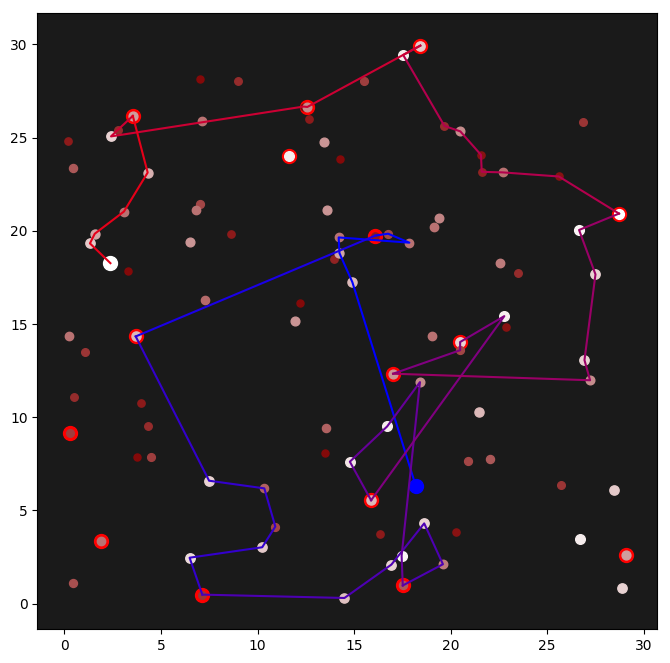
\includegraphics[width=\textwidth]{pictures/70.png}
    \caption{Example Solution: 100-200-15-10.ophsout}
    \label{fig:examplesol}
\end{figure}


\newpage

\section{Experiments}
After the first parts of the algorithm (file reading, file writing and error handling) were finished, a shell script was made to run the algorithm through every instance obtained from
\url{<https://www.mech.kuleuven.be/en/cib/op#section-14>}, so that thorough testing could be made with each increment in the algorithm's development. Before development of each phase started, the vertex and trip structures were created along with the functions that interact with them, so that any errors that could potentially disrupt data consistency would be contained and handled correctly before it could cause any havoc.

Finally, a python script was developed to plot each vertex given by the instance and the tour constructed by the algorithm, to visually see that it was working properly and as optimally as possible. Apart from this, some utility functions where created in the file $user\_io.c$ to print certain parts of the algorithm, like a trip's route or each vertices' location. After all of this was done, development on the actual algorithm started.

Before, during and after each phase described in the last section was developed, the program was tested with all instances and with different seeds, to assert that it was constantly functioning properly. Apart from this, the program was also debugged using the \textbf{Valgrind} tool to assert that memory was always being handled correctly.

A problem that appeared during the tour Greedy Randomized Construction phase was that for some instances of the problem none or only a small amount of viable solutions could be found. Due to the difficulty linked to designing an algorithm to repair these solutions while retaining good enough potential collected score, the invalid solutions were scraped at generation and the instances where no solutions could be found were scrapped.

After the algorithm's development finished, exhaustive testing was made with different values for each parameter by using the shell script mentioned before. The following conclusions were made by these tests regarding the parameters, along with a description of each:
\begin{itemize}
    \item \textbf{h\_rcl\_size}: As long as the \textbf{p\_rcl\_size} is kept between $5$ and $7$, \textbf{h\_rcl\_size} does not effect the results obtained greatly, as long as it's not $1$, which would make the hotel choice completely greedy. Values over $4$ are favoured tho, with $27$ out of the $32$ best-performing executions setting this parameter between $4$ and $10$. The default value was set to $9$, offering high exploration of wildly different solutions instead of stagnant exploitation of the same solutions over and over.
    \item \textbf{p\_rcl\_size}: As said before, values between $5$ and $7$ maximize the score collected by each solution, with $23$ out of the $32$ best-performing executions setting this parameter in that range. Due to the general size of the instances, this conclusion is logical, being a good enough point favoring exploration and exploitation equally. The default value was set to $5$, which accumulated the most best-performing executions ($9$ out of $32$) and being in the ``golden range'' described earlier.
    \item \textbf{ls\_iters\_n}: The average score collected by each tour was calculated for different values of this parameter, and this, along with the computation times, was used to set the default value to $15$, as the improvements after this value were less than $0.001\%$ and the increase in the computation time was no longer justified.
    \item \textbf{iters\_n}: As with \textbf{ls\_iter\_n}, the average score collected by each tour was calculated and was used alongside the computation times to decide on a default value, which was set at $5000$, since the improvements after this value were less than $2\%$ and the increase in the computation time was no longer acceptable.
\end{itemize}
The tests regarding \textbf{h\_rcl\_size} and \textbf{p\_rcl\_size} were made using an \textbf{iters\_n} of 100 and a \textbf{ls\_iters\_n} of 20, to be able to test with a relatively good speed, averaging out at $32103 [ms]$ for the compilation of the program and running on all the $405$ instances. Not much relation between the computation times and these values was perceived. Values for both parameters were tested between $1$ and $10$, going through each combination of the two parameters thorough this range. It is worth noting that the best performing combination of the two were $7$ for the hotel RCL and $5$ for the POI RCL.

After testing for the RCL sizes, the number of iterations for the Local Search phase were tested, keeping all the other parameters constant at 100 iterations and the RCL sizes set to the default values described before. Naturally, the value effects computation times significantly, shifting from $8203 [ms]$ when one iteration is used, to $125163 [ms]$ when a hundred iterations are used. The values for each \textbf{ls\_iters\_n} tested are shown in Table 3.

\begin{center}
    \begin{table}[]
    \centering
    \begin{tabular}{|r|r|r|}
        \hline
        \textbf{ls\_iter\_n} & impr. (\%) & comp. time [s] \\
        \hline
        $0$   & -       &   $6.968$ \\
        $1$   & $66.81$ &   $8.203$ \\
        $2$   & $7.95$  &   $9.685$ \\
        $3$   & $5.58$  &  $10.866$ \\
        $4$   & $3.57$  &  $12.127$ \\
        $5$   & $2.32$  &  $13.460$ \\
        $6$   & $1.26$  &  $14.933$ \\
        $7$   & $0.70$  &  $15.865$ \\
        $8$   & $0.34$  &  $17.223$ \\
        $9$   & $0.15$  &  $18.371$ \\
        $10$  & $0.09$  &  $19.721$ \\
        $11$  & $0.08$  &  $20.988$ \\
        $12$  & $0.02$  &  $22.006$ \\
        $13$  & $0.02$  &  $23.516$ \\
        $14$  & $0.00$  &  $24.978$ \\
        $15$  & $0.00$  &  $25.670$ \\
        $16$  & $0.00$  &  $27.143$ \\
        $17$  & $0.00$  &  $28.436$ \\
        $18$  & $0.00$  &  $29.488$ \\
        $19$  & $0.00$  &  $30.373$ \\
        $20$  & $0.00$  &  $31.727$ \\
        $50$  & $0.00$  &  $66.507$ \\
        $100$ & $0.00$  & $125.163$ \\
        \hline
    \end{tabular}
    \caption{Local Search Iterations Comparison}
    \label{ls\_iter\_n comparison}
    \end{table}
\end{center}

With all the other parameters set, testing for the number of iterations was fairly straightforward, trying varied values from $1$ to $10,000$ and analyzing the score improvement and computation time obtained with every value, comparing it to the one obtained with $1$ iteration. As with the number of iterations for the local search phase, the computation times were heavily influenced by increments in the number of iterations, going from $1933$ [ms] in one iteration to $2295233$ [ms] when $10,000$ iterations were ran. The values for each \textbf{iter\_n} tested and their results are shown in Table 4.

\begin{center}
    \begin{table}[]
    \centering
    \begin{tabular}{|r|r|r|}
        \hline
        \textbf{iter\_n} & impr. (\%) & comp. time [s] \\
        \hline
        $1$     &         &     $1.933$ \\
        $2$     & $56.16$ &     $2.240$ \\
        $5$     &  $5.47$ &     $3.115$ \\
        $10$    &  $4.30$ &     $4.344$ \\
        $20$    &  $3.92$ &     $6.798$ \\
        $50$    &  $5.13$ &    $13.986$ \\
        $100$   &  $3.56$ &    $26.004$ \\
        $200$   &  $3.66$ &    $50.064$ \\
        $500$   &  $3.55$ &   $137.272$ \\
        $1000$  &  $2.01$ &   $236.787$ \\
        $2000$  &  $2.30$ &   $484.299$ \\
        $5000$  &  $2.56$ & $1,155.956$ \\
        $10000$ &  $1.47$ & $2,295.233$ \\
        \hline
    \end{tabular}
    \caption{Number of Iterations Comparison}
    \label{iter\_n comparison}
    \end{table}
\end{center}

Finally, after the default value for the four parameters used was set, the robustness of the algorithm under different random seeds was tested. For this, all the parameters but the number of iterations were set at their default value, while \textbf{iter\_n} was set at $100$ so that testing could be done at a decent speed, since this value shouldn't effect the testing environment significantly.

The algorithm was ran with $20$ different seeds and the scaled standard deviation per instance was calculated by dividing the standard deviation by the mean for each instance. This value was plotted using the \textbf{MatPlotLib} library for the \textbf{Python 3} language, and the plot is shown in Figure 2.

%width=\textwidth

\begin{figure}
    \centering
    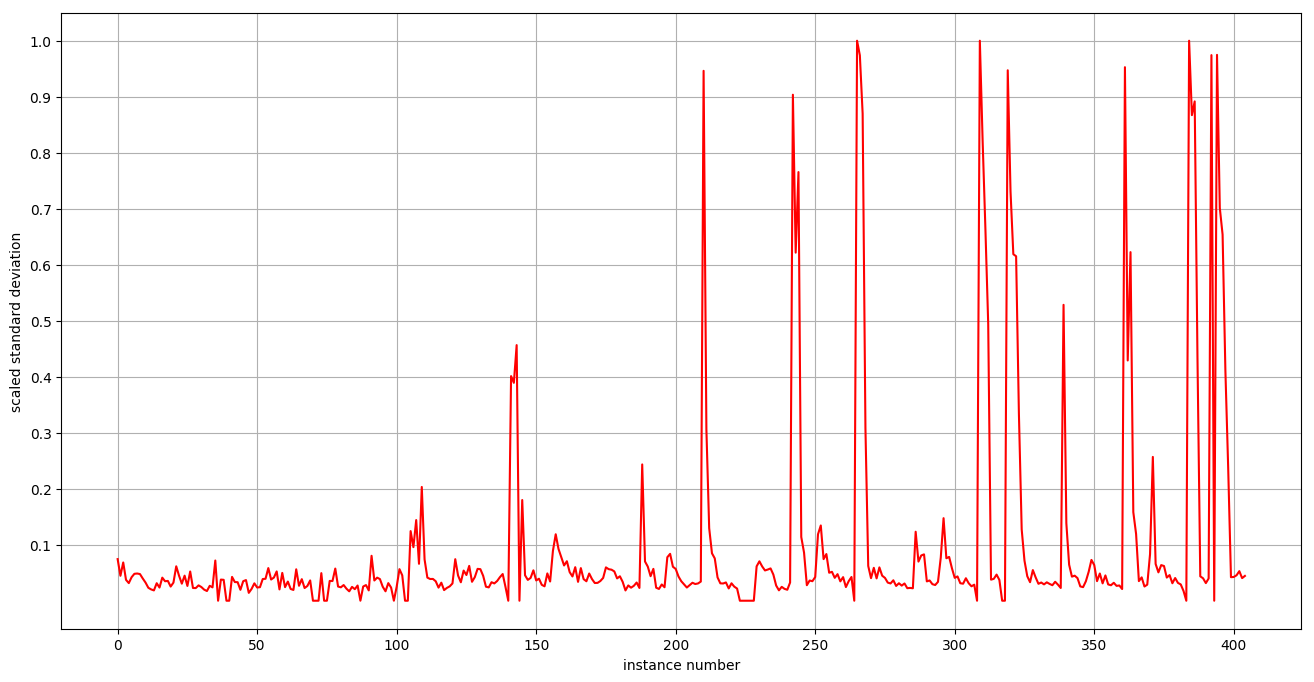
\includegraphics[scale=0.35]{pictures/stddev_graph.png}
    \caption{Scaled Standard Deviation for each Instance}
    \label{fig:stddevperinstance}
\end{figure}

From the graph, it can be seen that most of the instances have a scaled standard deviation of less than $0.1$, which speaks good about the robustness of the algorithm when looking at its independent behaviour from the random numbers given to it. It is worth noting that the occasional spikes, like on the last $13$ instances, is due to the problem mentioned before, that for some instances many solutions were scrapped in the tour Greedy Randomized Construction phase of the algorithm, leaving less solutions built in total and thus less variance between solutions. This is specially true for instances like ``$100-180-15-8\text{.ophs}$'' from ``SET$5\_15-8$'', where $3914$ iterations from the $5000$ ran produced no viable solutions.


\newpage

\section{Results}
In order to test the performance of the algorithm, it was tested on all previously available instances made in ~\cite{divsalar2013} and ~\cite{divsalar2014}. The implementation of the algorithm was written in pure \textbf{C}, the testing was done via \textbf{bash}, and the parameter tuning information was processed via \textbf{Python}, plotting with \textbf{MatPlotLib}. All the code base for the algorithm itself, the testing and plotting scripts can be accessed in \textbf{GitHub} under the \textbf{ophs\_grasp} repository (\url{<https://github.com/bleaktwig/ophs\_grasp>}), along with instructions to its correct use in the readme. All computations were carried out on a notebook Inter Core i5 6th-generation with $3.50$ GHz processor and $8.00$ GB RAM, with no parallelization.

The results are compared with the known optimal solution, along with the results of the skewed variable neighborhood search algorithm published in ~\cite{divsalar2013} and the memetic algorithms presented in ~\cite{divsalar2014}. A summary of these results is displayed in Table 5, where the first column shows the set of instances, the second column indicates the maximum TNFS in this set. Afterwards, the average percentage gap, the maximal percentage gap and the number of instances for which the optimal solution is found are displayed for the MA, SVNS and GRASP algorithms. Due to the randomness of the developed algorithm, it was applied on each instance three times. Finally, the average CPU time for the GRASP algorithm is displayed, comparing it to the average CPU time for the MA and SVNS algorithms. This results should be taken with a grain of salt, since these two algorithms were ran on a personal computer Intel Core 2 with $3.00$ GHz processor and $4.00$ GB RAM, providing less computational power than the one offered by the author's machine. The gap between the optimal result and the solution obtained by each algorithm is obtained in the following manner:
$100 \times \Big(\frac{\text{optimal result} - \text{algorithm result}}{optimal result}\Big)\%$. The results for each instance separately are shown in the Appendix A.

It is easy to see that the results obtained by the GRASP algorithm are very poor when compared to MA and SVNS. This deficiency is attributed to two main issues with the algorithm: First, simply that the local search phase doesn't have enough movements as to thoroughly go through the solution space to search for a good local optimum due to its very constrained solution neighborhood, and second, that the tour greedy construction search phase doesn't really contribute with good initial solutions anyway, working very randomly.

To fix these issues, it is planned to implement at least eight more movements to the local search phase to further improve the solutions and reach good local optima for each. The movements that are to be added are \textbf{Move-best}, \textbf{Two-Opt}, \textbf{Swap-trips}, \textbf{Extract-Insert}, \textbf{Extract2-Insert} \textbf{ExtractN-Insert}, \textbf{Extract-Move-Insert} and \textbf{Replacement}, which are the ones proven to be best for a TOP~\cite{divsalar2013}. Fixing the tour greedy construction phase is a harder task, since it's problem lies in it's design. Two solutions are hypothesized, adding a Repair phase after the tour GRC to improve the initial solutions and to fix the ones that are unfeasible from their conception, and simply scrapping the GRC approach to the generation of the tours, opting for a different algorithm inspired by how the Total Number of Feasible Sequences of Hotels affects the solutions found.

\begin{center}
    \begin{table}[]
    \centering
    \begin{adjustwidth}{-1in}{-1in}
    \begin{tabular}{|ll|lll|lll|lll|lll|}
\hline
\multicolumn{2}{|l}{} & \multicolumn{3}{|l}{MA} & \multicolumn{3}{|l}{SVNS} & \multicolumn{3}{|l}{GRASP} & \multicolumn{3}{|l|}{CPU Times} \\
\hline
Name & Max TNFS & Avg & Max & \# Opt & Avg & Max & \# Opt & Avg & Max & \# Opt & MA & SVNS & GRASP \\
1H2T  & $3                $ & $3.32$ & $13.91$ & $11$  & $1.22 $ & $7.55 $ & $18$  & $10.69$  & $22.95$  & $2$   & $1.84 $ & $0.12 $ & $2.02 $ \\
2H3T  & $16               $ & $0.88$ & $4.34 $ & $17$  & $0.93 $ & $5.19 $ & $19$  & $11.21$  & $24.02$  & $0$   & $1.43 $ & $0.14 $ & $2.04 $ \\
3H4T  & $125              $ & $0.60$ & $4.89 $ & $21$  & $0.92 $ & $5.00 $ & $18$  & $12.61$  & $27.89$  & $0$   & $1.09 $ & $0.41 $ & $1.91 $ \\
5H3T  & $49               $ & $0.81$ & $3.42 $ & $18$  & $0.93 $ & $4.05 $ & $19$  & $13.32$  & $26.70$  & $1$   & $1.41 $ & $0.21 $ & $1.64 $ \\
6H4T  & $512              $ & $0.64$ & $4.22 $ & $18$  & $1.21 $ & $5.19 $ & $17$  & $15.37$  & $27.76$  & $0$   & $1.15 $ & $0.88 $ & $1.63 $ \\
10H4T & $1728             $ & $1.72$ & $4.01 $ & $3 $  & $2.61 $ & $8.17 $ & $3 $  & $17.22$  & $25.59$  & $0$   & $6.59 $ & $5.12 $ & $5.19 $ \\
10H5T & $20736            $ & $1.99$ & $6.40 $ & $3 $  & $4.15 $ & $9.93 $ & $4 $  & $22.92$  & $46.60$  & $0$   & $5.43 $ & $4.26 $ & $4.59 $ \\
10H6T & $248832           $ & $2.30$ & $7.70 $ & $4 $  & $6.27 $ & $12.77$ & $4 $  & $25.56$  & $50.99$  & $0$   & $4.66 $ & $3.83 $ & $3.92 $ \\
12H4T & $2744             $ & $1.78$ & $5.16 $ & $5 $  & $2.73 $ & $6.08 $ & $2 $  & $17.93$  & $26.19$  & $0$   & $6.50 $ & $5.01 $ & $5.22 $ \\
12H5T & $38416            $ & $1.98$ & $5.15 $ & $4 $  & $3.58 $ & $8.68 $ & $4 $  & $21.82$  & $41.50$  & $0$   & $11.53$ & $8.73 $ & $8.13 $ \\
12H6T & $537824           $ & $2.28$ & $6.24 $ & $5 $  & $5.63 $ & $12.85$ & $3 $  & $24.33$  & $77.98$  & $0$   & $3.49 $ & $3.84 $ & $3.36 $ \\
15H4T & $4913             $ & $1.92$ & $5.15 $ & $3 $  & $2.66 $ & $5.76 $ & $2 $  & $16.53$  & $29.61$  & $0$   & $6.63 $ & $4.95 $ & $5.03 $ \\
15H5T & $83521            $ & $2.22$ & $4.42 $ & $3 $  & $4.42 $ & $11.52$ & $4 $  & $20.63$  & $41.99$  & $0$   & $5.41 $ & $4.20 $ & $4.22 $ \\
15H6T & $1419857          $ & $2.55$ & $6.11 $ & $4 $  & $6.86 $ & $13.52$ & $4 $  & $24.54$  & $59.33$  & $0$   & $4.78 $ & $4.29 $ & $3.47 $ \\
15H8T & $410338673        $ & $3.66$ & $9.75 $ & $1 $  & $15.54$ & $22.37$ & $0 $  & $32.49$  & $44.12$  & $0$   & $5.16 $ & $53.62$ & $1.42 $ \\
15H10T& $1.19\times10^{11}$ & $5.03$ & $9.25 $ & $1 $  & $-    $ & $-    $ & $0 $  & $38.57$  & $55.28$  & $0$   & $5.04 $ & $-    $ & $0.19 $ \\
SET4  & $25               $ & $7.38$ & $23.66$ & $4 $  & $7.44 $ & $23.66$ & $4 $  & $22.24$  & $26.06$  & $0$   & $1.17 $ & $0.24 $ & $3.93 $ \\
\hline
    \end{tabular}
    \end{adjustwidth}
    \caption{Experiments Results}
    \label{results}
    \end{table}
\end{center}

\newpage

\section{Concluding Remarks}
In this paper, the hotel selection variant of the orienteering problem is reviewed and two of the solutions found about the problem are closely examined, the Skewed Variable Neighbourhood Search method formulated in the original publication for the problem~\cite{divsalar2013}, and a Memetic Algorithm proposed by the same author a year later~\cite{divsalar2014}. Apart from this, the original orienteering problem is shortly explained, along with the team orienteering problem and the travelling salesman problem with hotel selections, due to the lack of publications regarding the OPHS by itself and how similar these three problems are to it. Algorithms for the OP, TOP and TSPHS are also reviewed, and a short description on how to adapt these algorithms for the OPHS is given as well.

An important factor about the OPHS is how the Total Number of Feasible Sequences of Hotels (TNFS) affects the execution time of any proposed algorithm to solve it. The maximal value of it for any instance is naturally equal to $H^{T-1}$, but the actual value can be much lower, and can be found using the initialization technique of the SVNS proposed by~\cite{divsalar2013}. Some graphs are given by~\cite{divsalar2014}, comparing the execution time and the average gap between the solutions found and the optimal solutions with the TNFS.

Another point worth noting is that, even if simple to develop, as of the current date nobody has published a simple multi-level greedy algorithm to find solutions for the problem. This algorithm would be beneficial to the research of the OPHS, since it would provide easy to compute solutions for any given instances as a benchmark to compare other algorithms too. Another point to consider is that no heuristic has challenged the problem that didn't use a multi-level approach, like the P-LS heuristic that managed to get astounding results for the TSPHS in incredibly low computation times due to how it didn't approach the problem in a multi-level fashion.

Many factors from other publications regarding the problem were taken into consideration while developing the algorithm for solving it. It is also worth noting that, while not very advanced, this is the first GRASP algorithm developed to tackle the OPHS, and with some more polishing it could potentially compete with the current best algorithms in the academy.

For future works concerning the problem, it is proposed to extend the OPHS with usual extensions of the OP, like time windows, route scores or various vehicles. Another simple extension would be to add a score to each hotel based on facilities, price or place. The development of a fast algorithm to calculate the TNFS for each instance would also be beneficial for the development of more research concerning the OPHS. Apart from this, an study on the problem to find its integer friendliness~\cite{revelle1993} would also be beneficial to improve the Mixed-Integer Linear Programming (MILP) algorithms developed to tackle it.

For future work concerning the algorithm, its improvement is the first thing that comes to mind. The tour Greedy Randomized Construction phase could be greatly improved by investing more computing time in pre-calculating how useful each trip could be before actually building them, along with the addition of a new Repair phase to work on fixing the currently scrapped solutions mentioned in Section 7. Apart from this, more movement will be added to the Local Search phase to have it explore more neighborhoods, and a path-relinking heuristic will be added to it to further improve the solutions using information found on solutions from previous iterations. Finding a non-multi-level approach to the problem is also considered for future work, considering the success of the P-LS heuristic mentioned before for the TSPHS.

\section{Appendix A. Detailed Results}
A set of tables containing the detailed results of the algorithm follow. The description for each column of the tables is in Section 8, with the small change that \textbf{G-Best}, \textbf{G-Avg} and \textbf{G-CPU} replace \textbf{GRASP-Best}, \textbf{GRASP-Avg} and \textbf{GRASP-CPU} from the summary table in that section.

\begin{center}
    \begin{table}[]
    \centering
    \begin{adjustwidth}{-0.4in}{-1in}
    \begin{tabular}{|lll|l|l|ll|lll|}
\hline
Name     & TNFS   & OPT  & MA-Avg & SVNS-Avg & G-Best & G-Avg & MA-CPU & SVNS-CPU & G-CPU \\
\hline
T1\_65   & $3$    & $240$  & $2.08$   & $\bm{0.00}$     & $14.58$      & $14.58$     & $0.40$   & $0.04$     & $0.81$      \\
T1\_70   & $3$    & $260$  & $5.77$   & $\bm{0.00}$     & $7.69 $      & $8.46 $     & $0.46$   & $0.04$     & $0.84$      \\
T1\_73   & $3$    & $265$  & $\bm{0.00}$   & $7.55$     & $11.32$      & $12.08$     & $0.43$   & $0.03$     & $0.86$      \\
T1\_75   & $3$    & $270$  & $\bm{0.00}$   & $\bm{0.00}$     & $\bm{0.00} $      & $5.56 $     & $0.38$   & $0.03$     & $0.86$      \\
T1\_80   & $3$    & $280$  & $3.57$   & $3.57$     & $3.57 $      & $4.64 $     & $0.42$   & $0.03$     & $0.88$      \\
T1\_85   & $3$    & $285$  & $\bm{0.00}$   & $1.75$     & $1.75 $      & $2.81 $     & $0.37$   & $0.04$     & $0.88$      \\
\hline
T3\_65   & $3$    & $610$  & $\bm{0.00}$   & $\bm{0.00}$     & $6.56$       & $6.56 $     & $0.42$   & $0.04$     & $0.88$      \\
T3\_75   & $3$    & $670$  & $\bm{0.00}$   & $2.99$     & $7.46$       & $7.76 $     & $0.45$   & $0.03$     & $0.88$      \\
T3\_80   & $3$    & $710$  & $0.94$   & $2.82$     & $8.45$       & $11.27$     & $0.46$   & $0.04$     & $0.91$      \\
T3\_85   & $3$    & $740$  & $4.05$   & $\bm{0.00}$     & $9.46$       & $9.86 $     & $0.34$   & $0.03$     & $0.91$      \\
T3\_90   & $3$    & $770$  & $\bm{0.00}$   & $\bm{0.00}$     & $7.79$       & $8.70 $     & $0.37$   & $0.04$     & $0.92$      \\
T3\_95   & $3$    & $790$  & $\bm{0.00}$   & $1.27$     & $8.86$       & $8.86 $     & $0.37$   & $0.03$     & $0.93$      \\
T3\_100  & $3$    & $800$  & $6.25$   & $3.75$     & $10.00$      & $10.00$     & $0.41$   & $0.03$     & $0.91$      \\
T3\_105  & $3$    & $800$  & $0.42$   & $\bm{0.00}$     & $3.75$       & $4.62 $     & $0.32$   & $0.03$     & $0.96$      \\
\hline
64\_45   & $3$    & $816 $ & $9.56$   & $\bm{0.00}$     & $22.79$      & $23.53$     & $3.48$   & $0.19$     & $3.28$      \\
64\_50   & $3$    & $900 $ & $3.33$   & $2.67$     & $15.33$      & $22.67$     & $3.01$   & $0.26$     & $3.23$      \\
64\_55   & $3$    & $984 $ & $2.44$   & $1.22$     & $14.02$      & $14.63$     & $3.60$   & $0.24$     & $3.13$      \\
64\_60   & $3$    & $1062$ & $3.58$   & $1.13$     & $15.25$      & $15.63$     & $5.44$   & $0.27$     & $2.98$      \\
64\_65   & $3$    & $1116$ & $0.72$   & $\bm{0.00}$     & $11.83$      & $12.37$     & $5.96$   & $0.29$     & $2.85$      \\
64\_70   & $3$    & $1188$ & $2.53$   & $1.52$     & $11.62$      & $11.95$     & $4.60$   & $0.24$     & $2.77$      \\
64\_75   & $3$    & $1236$ & $2.10$   & $\bm{0.00}$     & $8.74 $      & $9.22 $     & $4.17$   & $0.29$     & $2.63$      \\
64\_80   & $3$    & $1284$ & $2.18$   & $\bm{0.00}$     & $6.54 $      & $8.41 $     & $4.71$   & $0.24$     & $2.44$      \\
\hline
66\_40   & $3$    & $575 $ & $13.91$  & $0.87$     & $20.00$      & $21.74$     & $1.31$   & $0.09$     & $1.99$      \\
66\_45   & $3$    & $650 $ & $8.46 $  & $0.77$     & $17.69$      & $18.46$     & $1.29$   & $0.11$     & $2.14$      \\
66\_50   & $3$    & $730 $ & $4.11 $  & $2.05$     & $22.60$      & $23.29$     & $2.55$   & $0.12$     & $2.28$      \\
66\_55   & $3$    & $825 $ & $4.04 $  & $2.42$     & $20.00$      & $23.64$     & $1.36$   & $0.16$     & $2.37$      \\
66\_60   & $3$    & $915 $ & $10.02$  & $6.01$     & $22.95$      & $25.03$     & $2.13$   & $0.20$     & $2.51$      \\
66\_125  & $3$    & $1670$ & $1.80 $  & $0.30$     & $6.59 $      & $7.07 $     & $3.93$   & $0.22$     & $3.70$      \\
66\_130  & $3$    & $1680$ & $\bm{0.00} $  & $\bm{0.00}$     & $4.46 $      & $5.95 $     & $3.88$   & $0.24$     & $3.79$      \\
\hline
100\_30  & $2$    & $173$  & $5.78$   & $\bm{0.00}$     & $13.87$      & $13.87$     & $0.40$   & $0.03$     & $2.17$      \\
100\_35  & $1$    & $241$  & $\bm{0.00}$   & $\bm{0.00}$     & $7.05 $      & $12.45$     & $0.78$   & $0.06$     & $2.89$      \\
100\_40  & $2$    & $299$  & $\bm{0.00}$   & $\bm{0.00}$     & $11.04$      & $11.04$     & $0.68$   & $0.14$     & $3.10$      \\
100\_45  & $3$    & $367$  & $\bm{0.00}$   & $\bm{0.00}$     & $13.08$      & $14.44$     & $1.28$   & $0.12$     & $3.35$      \\
\hline
102\_50  & $3$    & $181$  & $11.05$  & $\bm{0.00}$     & $\bm{0.00}$       & $\bm{0.00}$      & $0.25$   & $0.02$     & $2.18$      \\
102\_60  & $3$    & $243$  & $7.41 $  & $\bm{0.00}$     & $7.41$       & $7.82$      & $0.51$   & $0.05$     & $2.64$      \\
\hline
Average & $2.89$  & $-$    & $3.32 $  & $1.22$     & $10.69$      & $11.97$     & $1.74$   & $0.12$     & $2.02$      \\
Max     & $3   $  & $-$    & $13.91$  & $7.55$     & $22.95$      & $25.03$     & $5.96$   & $0.29$     & $3.79$      \\
\hline
    \end{tabular}
    \end{adjustwidth}
    \caption{1 Extra hotel 2 Trips}
    \label{1-2}
    \end{table}
\end{center}
\begin{center}
    \begin{table}[]
    \centering
    \begin{adjustwidth}{-0.4in}{-1in}
    \begin{tabular}{|lll|l|l|ll|lll|}
\hline
Name     & TNFS   & OPT    & MA-Avg   &SVNS-Avg& G-Best  & G-Avg   & MA-CPU   & SVNS-CPU   & G-CPU \\
\hline
T1\_65   & $16  $ & $240 $ & $\bm{0.00}  $ & $\bm{0.00}$ & $10.42$ & $10.42$ & $0.39  $ & $0.05    $ & $0.84     $ \\
T1\_70   & $16  $ & $260 $ & $\bm{0.00}  $ & $\bm{0.00}$ & $19.23$ & $19.23$ & $0.41  $ & $0.04    $ & $0.84     $ \\
T1\_73   & $16  $ & $265 $ & $\bm{0.00}  $ & $\bm{0.00}$ & $20.75$ & $22.64$ & $0.45  $ & $0.04    $ & $0.84     $ \\
T1\_75   & $16  $ & $270 $ & $\bm{0.00}  $ & $\bm{0.00}$ & $7.41 $ & $8.52 $ & $0.36  $ & $0.07    $ & $0.84     $ \\
T1\_80   & $16  $ & $280 $ & $\bm{0.00}  $ & $\bm{0.00}$ & $10.71$ & $11.43$ & $0.39  $ & $0.04    $ & $0.83     $ \\
T1\_85   & $16  $ & $285 $ & $\bm{0.00}  $ & $\bm{0.00}$ & $3.51 $ & $4.21 $ & $0.46  $ & $0.05    $ & $0.86     $ \\
\hline
T3\_65   & $16  $ & $610 $ & $1.09  $ & $\bm{0.00}$ & $8.20 $ & $8.69 $ & $0.39  $ & $0.04    $ & $0.86     $ \\
T3\_75   & $16  $ & $670 $ & $\bm{0.00}  $ & $2.99$ & $5.97 $ & $6.42 $ & $0.48  $ & $0.05    $ & $0.88     $ \\
T3\_80   & $16  $ & $710 $ & $\bm{0.00}  $ & $\bm{0.00}$ & $5.63 $ & $6.06 $ & $0.44  $ & $0.05    $ & $0.90     $ \\
T3\_85   & $16  $ & $740 $ & $2.70  $ & $\bm{0.00}$ & $8.11 $ & $8.11 $ & $0.43  $ & $0.07    $ & $0.90     $ \\
T3\_90   & $16  $ & $770 $ & $1.30  $ & $5.19$ & $11.69$ & $12.99$ & $0.38  $ & $0.05    $ & $0.88     $ \\
T3\_95   & $16  $ & $790 $ & $\bm{0.00}  $ & $\bm{0.00}$ & $6.33 $ & $6.71 $ & $0.49  $ & $0.06    $ & $0.90     $ \\
T3\_100  & $16  $ & $800 $ & $\bm{0.00}  $ & $\bm{0.00}$ & $6.25 $ & $6.62 $ & $0.40  $ & $0.05    $ & $0.88     $ \\
T3\_105  & $16  $ & $800 $ & $0.83  $ & $1.25$ & $5.00 $ & $5.88 $ & $0.43  $ & $0.05    $ & $0.89     $ \\
\hline
64\_45   & $16  $ & $816 $ & $1.47  $ & $\bm{0.00}$ & $23.53$ & $24.02$ & $1.55  $ & $0.18    $ & $2.51     $ \\
64\_50   & $16  $ & $900 $ & $3.33  $ & $2.67$ & $13.33$ & $14.44$ & $1.98  $ & $0.25    $ & $2.68     $ \\
64\_55   & $16  $ & $984 $ & $2.85  $ & $3.05$ & $7.93 $ & $10.16$ & $2.40  $ & $0.26    $ & $2.88     $ \\
64\_60   & $16  $ & $1062$ & $\bm{0.00}  $ & $2.26$ & $12.43$ & $12.99$ & $2.64  $ & $0.44    $ & $2.95     $ \\
64\_65   & $16  $ & $1116$ & $0.18  $ & $2.15$ & $11.29$ & $11.29$ & $3.71  $ & $0.33    $ & $3.08     $ \\
64\_70   & $16  $ & $1188$ & $1.68  $ & $1.52$ & $13.13$ & $13.30$ & $4.30  $ & $0.39    $ & $3.22     $ \\
64\_75   & $16  $ & $1236$ & $2.10  $ & $1.94$ & $8.74 $ & $9.06 $ & $4.96  $ & $0.34    $ & $3.26     $ \\
64\_80   & $16  $ & $1284$ & $2.34  $ & $1.87$ & $4.67 $ & $6.54 $ & $4.69  $ & $0.35    $ & $3.23     $ \\
\hline
66\_40   & $16  $ & $575 $ & $0.87  $ & $0.87$ & $13.04$ & $14.26$ & $0.84  $ & $0.08    $ & $2.29     $ \\
66\_45   & $16  $ & $650 $ & $0.77  $ & $0.77$ & $6.15 $ & $6.62 $ & $0.72  $ & $0.09    $ & $2.37     $ \\
66\_50   & $16  $ & $730 $ & $4.34  $ & $2.05$ & $8.22 $ & $9.32 $ & $1.02  $ & $0.15    $ & $2.52     $ \\
66\_55   & $16  $ & $825 $ & $1.62  $ & $2.42$ & $10.30$ & $12.73$ & $1.40  $ & $0.16    $ & $2.61     $ \\
66\_60   & $16  $ & $915 $ & $1.64  $ & $0.55$ & $18.03$ & $18.80$ & $1.59  $ & $0.19    $ & $2.69     $ \\
66\_125  & $16  $ & $1670$ & $1.40  $ & $\bm{0.00}$ & $9.58 $ & $10.06$ & $4.95  $ & $0.37    $ & $3.50     $ \\
66\_130  & $16  $ & $1680$ & $0.30  $ & $0.89$ & $7.14 $ & $8.63 $ & $4.84  $ & $0.30    $ & $3.52     $ \\
\hline
100\_30  & $1   $ & $173 $ & $\bm{0.00}  $ & $\bm{0.00}$ & $5.20 $ & $6.94 $ & $0.34  $ & $0.02    $ & $2.18     $ \\
100\_35  & $2   $ & $241 $ & $\bm{0.00}  $ & $\bm{0.00}$ & $-    $ & $-    $ & $0.48  $ & $0.05    $ & $-        $ \\
100\_40  & $2   $ & $299 $ & $\bm{0.00}  $ & $\bm{0.00}$ & $9.03 $ & $9.03 $ & $0.53  $ & $0.04    $ & $3.57     $ \\
100\_45  & $2   $ & $367 $ & $\bm{0.00}  $ & $\bm{0.00}$ & $20.44$ & $22.62$ & $0.71  $ & $0.07    $ & $3.95     $ \\
\hline
102\_50  & $12  $ & $181 $ & $\bm{0.00}  $ & $\bm{0.00}$ & $-    $ & $-    $ & $0.15  $ & $0.02    $ & $-        $ \\
102\_60  & $12  $ & $243 $ & $\bm{0.00}  $ & $\bm{0.00}$ & $-    $ & $-    $ & $0.33  $ & $0.05    $ & $-        $ \\
\hline
Average  & $14.4$ & $-   $ & $0.88  $ & $0.93$ & $10.36$ & $11.21$ & $1.43  $ & $0.14    $ & $2.04     $ \\
Max      & $16  $ & $-   $ & $4.34  $ & $5.19$ & $23.53$ & $24.02$ & $4.96  $ & $0.44    $ & $3.95     $ \\
\hline
\end{tabular}
    \end{adjustwidth}
    \caption{2 Extra hotels 3 Trips}
    \label{2-3}
    \end{table}
\end{center}
\begin{center}
    \begin{table}[]
    \centering
    \begin{adjustwidth}{-0.4in}{-1in}
    \begin{tabular}{|lll|l|l|ll|lll|}
\hline
Name    & TNFS    & OPT    & MA-Avg & SVNS-Avg & G-Best  & G-Avg   & MA-CPU & SVNS-CPU & G-CPU \\
\hline
T1\_65  & $107  $ & $240 $ & $\bm{0.00}$ & $\bm{0.00}$   & $18.75$ & $20.00$ & $0.28$ & $0.12$   & $0.46$ \\
T1\_70  & $107  $ & $260 $ & $\bm{0.00}$ & $\bm{0.00}$   & $7.69$  & $7.69$  & $0.31$ & $0.12$   & $0.46$ \\
T1\_73  & $107  $ & $265 $ & $\bm{0.00}$ & $\bm{0.00}$   & $5.66$  & $5.66$  & $0.32$ & $0.12$   & $0.45$ \\
T1\_75  & $107  $ & $270 $ & $\bm{0.00}$ & $\bm{0.00}$   & $27.78$ & $27.78$ & $0.35$ & $0.12$   & $0.46$ \\
T1\_80  & $125  $ & $280 $ & $\bm{0.00}$ & $1.79$   & $14.29$ & $15.00$ & $0.36$ & $0.17$   & $0.89$ \\
T1\_85  & $125  $ & $285 $ & $\bm{0.00}$ & $\bm{0.00}$   & $8.77$  & $9.82$  & $0.37$ & $0.15$   & $0.89$ \\
\hline
T3\_65  & $100  $ & $610 $ & $\bm{0.00}$ & $\bm{0.00}$   & $-$     & $-$     & $0.33$ & $0.12$   & $-   $ \\
T3\_75  & $125  $ & $670 $ & $\bm{0.00}$ & $2.99$   & $11.94$ & $12.99$ & $0.34$ & $0.16$   & $0.97$ \\
T3\_80  & $107  $ & $710 $ & $\bm{0.00}$ & $\bm{0.00}$   & $15.49$ & $15.49$ & $0.31$ & $0.14$   & $0.48$ \\
T3\_85  & $107  $ & $740 $ & $\bm{0.00}$ & $\bm{0.00}$   & $12.16$ & $14.86$ & $0.34$ & $0.14$   & $0.48$ \\
T3\_90  & $100  $ & $770 $ & $\bm{0.00}$ & $\bm{0.00}$   & $-$     & $-$     & $0.37$ & $0.21$   & $-   $ \\
T3\_95  & $100  $ & $790 $ & $\bm{0.00}$ & $\bm{0.00}$   & $-$     & $-$     & $0.44$ & $0.15$   & $-   $ \\
T3\_100 & $125  $ & $800 $ & $\bm{0.00}$ & $5.00$   & $15.00$ & $15.88$ & $0.38$ & $0.19$   & $0.94$ \\
T3\_105 & $125  $ & $800 $ & $0.42$ & $\bm{0.00}$   & $7.50$  & $8.38$  & $0.41$ & $0.20$   & $0.90$ \\
\hline
64\_45  & $44   $ & $816 $ & $\bm{0.00}$ & $\bm{0.00}$   & $5.88$  & $9.07$  & $1.33$ & $0.18$   & $1.42$ \\
64\_50  & $72   $ & $900 $ & $4.89$ & $3.33$   & $14.67$ & $15.56$ & $1.64$ & $0.61$   & $2.91$ \\
64\_55  & $100  $ & $984 $ & $0.61$ & $0.61$   & $11.59$ & $13.21$ & $1.56$ & $0.94$   & $3.00$ \\
64\_60  & $100  $ & $1062$ & $1.88$ & $2.26$   & $10.17$ & $14.31$ & $2.09$ & $0.75$   & $3.07$ \\
64\_65  & $125  $ & $1116$ & $0.36$ & $1.08$   & $11.29$ & $12.19$ & $2.51$ & $1.04$   & $3.17$ \\
64\_70  & $125  $ & $1188$ & $2.19$ & $1.52$   & $12.63$ & $13.13$ & $2.88$ & $1.71$   & $3.21$ \\
64\_75  & $125  $ & $1236$ & $2.91$ & $2.91$   & $7.77$  & $8.74$  & $2.78$ & $1.24$   & $3.18$ \\
64\_80  & $125  $ & $1284$ & $0.93$ & $1.40$   & $9.81$  & $10.12$ & $3.71$ & $1.39$   & $3.19$ \\
\hline
66\_40  & $107  $ & $575 $ & $0.87$ & $0.87$   & $15.65$ & $15.65$ & $0.46$ & $0.16$   & $1.31$ \\
66\_45  & $88   $ & $650 $ & $0.77$ & $0.77$   & $-$     & $-$     & $0.74$ & $0.19$   & $-   $ \\
66\_50  & $107  $ & $730 $ & $2.05$ & $2.05$   & $6.16$  & $6.85$  & $0.83$ & $0.31$   & $2.84$ \\
66\_55  & $107  $ & $825 $ & $\bm{0.00}$ & $2.42$   & $5.45$  & $5.82$  & $0.92$ & $0.37$   & $2.95$ \\
66\_60  & $107  $ & $915 $ & $0.55$ & $0.55$   & $5.46$  & $6.01$  & $1.11$ & $0.44$   & $3.00$ \\
66\_125 & $125  $ & $1670$ & $1.70$ & $2.10$   & $21.86$ & $23.35$ & $4.47$ & $1.43$   & $3.42$ \\
66\_130 & $125  $ & $1680$ & $0.89$ & $0.60$   & $11.61$ & $12.98$ & $4.16$ & $1.39$   & $3.39$ \\
\hline
100\_30 & $2    $ & $173 $ & $\bm{0.00}$ & $\bm{0.00}$   & $-$     & $-$     & $0.36$ & $0.03$   & $-   $ \\
100\_35 & $1    $ & $241 $ & $\bm{0.00}$ & $\bm{0.00}$   & $-$     & $-$     & $0.29$ & $0.03$   & $-   $ \\
100\_40 & $1    $ & $299 $ & $\bm{0.00}$ & $\bm{0.00}$   & $-$     & $-$     & $0.52$ & $0.04$   & $-   $ \\
100\_45 & $2    $ & $367 $ & $\bm{0.00}$ & $\bm{0.00}$   & $5.45$  & $7.36$  & $0.50$ & $0.05$   & $2.28$ \\
\hline
102\_50 & $33   $ & $181 $ & $\bm{0.00}$ & $\bm{0.00}$   & $-$     & $-$     & $0.15$ & $0.03$   & $-   $ \\
102\_60 & $60   $ & $243 $ & $\bm{0.00}$ & $\bm{0.00}$   & $-$     & $-$     & $0.34$ & $0.05$   & $-   $ \\
\hline
Average & $92.80$ & $-   $ & $0.60$ & $0.92$   & $11.56$ & $12.61$ & $1.09$ & $0.41$   & $1.91$ \\
Max     & $125  $ & $-   $ & $4.89$ & $5.00$   & $27.78$ & $27.78$ & $4.47$ & $1.71$   & $3.42$ \\
\hline
\end{tabular}
    \end{adjustwidth}
    \caption{3 Extra hotels 4 Trips}
    \label{3-4}
    \end{table}
\end{center}
\begin{center}
    \begin{table}[]
    \centering
    \begin{adjustwidth}{-0.4in}{-1in}
    \begin{tabular}{|lll|l|l|ll|lll|}
\hline
Name    & TNFS    & OPT    & MA-Avg &SVNS-Avg& G-Best  & G-Avg   & MA-CPU & SVNS-CPU & G-CPU \\
\hline
T1\_65   & $49  $ & $240 $ & $\bm{0.00}$ & $\bm{0.00}$ & $10.42$ & $10.42$ & $0.07$ & $0.07$   & $0.84$ \\
T1\_70   & $49  $ & $260 $ & $0.64$ & $\bm{0.00}$ & $13.46$ & $14.23$ & $0.07$ & $0.07$   & $0.84$ \\
T1\_73   & $49  $ & $265 $ & $\bm{0.00}$ & $\bm{0.00}$ & $16.98$ & $16.98$ & $0.07$ & $0.07$   & $0.83$ \\
T1\_75   & $49  $ & $270 $ & $\bm{0.00}$ & $\bm{0.00}$ & $9.26$  & $9.26$  & $0.10$ & $0.10$   & $0.83$ \\
T1\_80   & $49  $ & $280 $ & $\bm{0.00}$ & $\bm{0.00}$ & $10.71$ & $11.79$ & $0.07$ & $0.07$   & $0.84$ \\
T1\_85   & $49  $ & $285 $ & $\bm{0.00}$ & $\bm{0.00}$ & $7.02$  & $8.07$  & $0.08$ & $0.08$   & $0.85$ \\
\hline
T3\_65   & $49  $ & $610 $ & $\bm{0.00}$ & $\bm{0.00}$ & $14.75$ & $15.25$ & $0.09$ & $0.09$   & $0.86$ \\
T3\_75   & $49  $ & $670 $ & $2.49$ & $2.99$ & $7.46$  & $7.46$  & $0.08$ & $0.08$   & $0.89$ \\
T3\_80   & $49  $ & $710 $ & $\bm{0.00}$ & $\bm{0.00}$ & $8.45$  & $12.68$ & $0.08$ & $0.08$   & $0.89$ \\
T3\_85   & $49  $ & $740 $ & $2.70$ & $4.05$ & $12.16$ & $12.16$ & $0.08$ & $0.08$   & $0.89$ \\
T3\_90   & $49  $ & $770 $ & $\bm{0.00}$ & $3.90$ & $9.09$  & $12.60$ & $0.08$ & $0.08$   & $0.88$ \\
T3\_95   & $49  $ & $790 $ & $\bm{0.00}$ & $\bm{0.00}$ & $10.13$ & $11.01$ & $0.09$ & $0.09$   & $0.89$ \\
T3\_100  & $49  $ & $800 $ & $\bm{0.00}$ & $\bm{0.00}$ & $8.75$  & $10.00$ & $0.08$ & $0.08$   & $0.90$ \\
T3\_105  & $49  $ & $800 $ & $\bm{0.00}$ & $\bm{0.00}$ & $5.00$  & $5.88$  & $0.08$ & $0.08$   & $0.88$ \\
\hline
64\_45   & $49  $ & $816 $ & $0.98$ & $\bm{0.00}$ & $21.32$ & $23.28$ & $0.26$ & $0.26$   & $2.58$ \\
64\_50   & $49  $ & $900 $ & $2.89$ & $3.33$ & $14.67$ & $16.00$ & $0.37$ & $0.37$   & $2.74$ \\
64\_55   & $49  $ & $984 $ & $3.05$ & $3.05$ & $12.80$ & $14.43$ & $0.42$ & $0.42$   & $2.96$ \\
64\_60   & $49  $ & $1062$ & $0.75$ & $0.56$ & $13.56$ & $13.75$ & $0.48$ & $0.48$   & $2.94$ \\
64\_65   & $49  $ & $1116$ & $1.08$ & $2.15$ & $9.68$  & $11.47$ & $0.54$ & $0.54$   & $3.02$ \\
64\_70   & $49  $ & $1188$ & $1.85$ & $1.52$ & $10.10$ & $11.28$ & $0.57$ & $0.57$   & $3.10$ \\
64\_75   & $49  $ & $1236$ & $1.62$ & $1.46$ & $6.80$  & $8.90$  & $0.62$ & $0.62$   & $3.51$ \\
64\_80   & $49  $ & $1284$ & $1.40$ & $1.87$ & $8.88$  & $9.35$  & $0.58$ & $0.58$   & $3.48$ \\
\hline
66\_40   & $45  $ & $575 $ & $0.87$ & $0.87$ & $14.78$ & $16.17$ & $0.11$ & $0.11$   & $2.09$ \\
66\_45   & $47  $ & $650 $ & $0.77$ & $0.77$ & $16.92$ & $18.46$ & $0.16$ & $0.16$   & $2.42$ \\
66\_50   & $49  $ & $730 $ & $3.42$ & $2.05$ & $21.23$ & $21.51$ & $0.22$ & $0.22$   & $2.55$ \\
66\_55   & $49  $ & $825 $ & $\bm{0.00}$ & $\bm{0.00}$ & $18.18$ & $20.00$ & $0.40$ & $0.40$   & $2.66$ \\
66\_60   & $49  $ & $915 $ & $2.37$ & $2.73$ & $21.31$ & $22.95$ & $0.30$ & $0.30$   & $2.77$ \\
66\_125  & $49  $ & $1670$ & $0.80$ & $0.90$ & $8.68$  & $11.20$ & $0.53$ & $0.53$   & $3.44$ \\
66\_130  & $49  $ & $1680$ & $0.50$ & $0.30$ & $8.93$  & $10.60$ & $0.54$ & $0.54$   & $3.44$ \\
\hline
100\_30  & $1   $ & $173 $ & $\bm{0.00}$ & $\bm{0.00}$ & $15.03$ & $15.61$ & $0.02$ & $0.02$   & $0.20$ \\
100\_35  & $2   $ & $241 $ & $\bm{0.00}$ & $\bm{0.00}$ & $17.43$ & $17.43$ & $0.05$ & $0.05$   & $0.30$ \\
100\_40  & $2   $ & $299 $ & $\bm{0.00}$ & $\bm{0.00}$ & $12.04$ & $12.04$ & $0.05$ & $0.05$   & $0.31$ \\
100\_45  & $2   $ & $367 $ & $\bm{0.00}$ & $\bm{0.00}$ & $26.70$ & $26.70$ & $0.07$ & $0.07$   & $0.35$ \\
\hline
102\_50  & $14  $ & $181 $ & $\bm{0.00}$ & $\bm{0.00}$ & $\bm{0.00}$  & $\bm{0.00}$  & $0.02$ & $0.02$   & $0.18$ \\
102\_60  & $17  $ & $243 $ & $\bm{0.00}$ & $\bm{0.00}$ & $7.41$  & $7.41$  & $0.05$ & $0.05$   & $0.26$ \\
\hline
Average & $41.51$ & $-   $ & $0.81$ & $0.93$ & $12.29$ & $13.32$ & $0.21$ & $0.21$   & $1.64$ \\
Max     & $49   $ & $-   $ & $3.42$ & $4.05$ & $26.70$ & $26.70$ & $0.62$ & $0.62$   & $3.51$ \\
\hline
\end{tabular}
    \end{adjustwidth}
    \caption{5 Extra hotels 3 Trips}
    \label{5-3}
    \end{table}
\end{center}
\begin{center}
    \begin{table}[]
    \centering
    \begin{adjustwidth}{-0.4in}{-1in}
    \begin{tabular}{|lll|l|l|ll|lll|}
\hline
Name    & TNFS    & OPT    & MA-Avg & SVNS-Avg & G-Best   & G-Avg   & MA-CPU & SVNS-CPU & G-CPU \\
\hline
T1\_65  & $482   $& $240 $ & $\bm{0.00}$ & $\bm{0.00}$   & $12.50$  & $13.33$ & $0.27$ & $0.27$ & $0.89$ \\
T1\_70  & $482   $& $260 $ & $\bm{0.00}$ & $\bm{0.00}$   & $13.46$  & $16.54$ & $0.28$ & $0.28$ & $0.90$ \\
T1\_73  & $482   $& $265 $ & $1.26$ & $\bm{0.00}$   & $13.21$  & $13.21$ & $0.35$ & $0.35$ & $0.90$ \\
T1\_75  & $482   $& $270 $ & $\bm{0.00}$ & $\bm{0.00}$   & $9.26 $  & $10.37$ & $0.32$ & $0.32$ & $0.89$ \\
T1\_80  & $512   $& $280 $ & $1.19$ & $\bm{0.00}$   & $12.50$  & $16.79$ & $0.35$ & $0.35$ & $0.89$ \\
T1\_85  & $512   $& $285 $ & $\bm{0.00}$ & $\bm{0.00}$   & $10.53$  & $11.23$ & $0.33$ & $0.33$ & $0.89$ \\
\hline
T3\_65  & $448   $& $610 $ & $\bm{0.00}$ & $\bm{0.00}$   & $21.31$  & $22.95$ & $0.31$ & $0.31$ & $0.87$ \\
T3\_75  & $512   $& $670 $ & $\bm{0.00}$ & $2.99$   & $11.94$  & $12.99$ & $0.34$ & $0.34$ & $0.92$ \\
T3\_80  & $482   $& $710 $ & $\bm{0.00}$ & $\bm{0.00}$   & $12.68$  & $13.66$ & $0.34$ & $0.34$ & $0.95$ \\
T3\_85  & $482   $& $740 $ & $\bm{0.00}$ & $\bm{0.00}$   & $16.22$  & $17.16$ & $0.36$ & $0.36$ & $0.95$ \\
T3\_90  & $448   $& $770 $ & $\bm{0.00}$ & $5.19$   & $14.29$  & $15.58$ & $0.39$ & $0.39$ & $0.98$ \\
T3\_95  & $448   $& $790 $ & $\bm{0.00}$ & $5.06$   & $17.72$  & $18.10$ & $0.39$ & $0.39$ & $0.98$ \\
T3\_100 & $512   $& $800 $ & $\bm{0.00}$ & $5.00$   & $16.25$  & $17.50$ & $0.38$ & $0.38$ & $0.92$ \\
T3\_105 & $512   $& $800 $ & $0.42$ & $\bm{0.00}$   & $10.00$  & $11.25$ & $0.40$ & $0.40$ & $0.91$ \\
\hline
64\_45  & $252   $& $816 $ & $0.98$ & $2.94$   & $13.97$  & $17.65$ & $1.08$ & $1.08$ & $2.22$ \\
64\_50  & $378   $& $900 $ & $4.22$ & $3.33$   & $22.00$  & $24.00$ & $1.47$ & $1.47$ & $2.98$ \\
64\_55  & $448   $& $984 $ & $1.22$ & $1.22$   & $18.29$  & $19.11$ & $1.73$ & $1.73$ & $3.07$ \\
64\_60  & $448   $& $1062$ & $0.56$ & $1.69$   & $19.77$  & $20.90$ & $2.03$ & $2.03$ & $3.11$ \\
64\_65  & $512   $& $1116$ & $\bm{0.00}$ & $\bm{0.00}$   & $12.37$  & $13.26$ & $2.35$ & $2.35$ & $3.19$ \\
64\_70  & $512   $& $1188$ & $2.69$ & $2.02$   & $15.66$  & $16.50$ & $2.33$ & $2.33$ & $3.25$ \\
64\_75  & $512   $& $1236$ & $1.62$ & $2.91$   & $12.62$  & $13.27$ & $2.48$ & $2.48$ & $3.23$ \\
64\_80  & $512   $& $1284$ & $1.09$ & $1.40$   & $14.02$  & $15.58$ & $2.63$ & $2.63$ & $3.23$ \\
\hline
66\_40  & $302   $& $575 $ & $0.87$ & $0.87$   & $9.57 $  & $9.91$  & $0.41$ & $0.41$ & $1.60$ \\
66\_45  & $228   $& $650 $ & $0.77$ & $0.77$   & $8.46 $  & $10.31$ & $0.54$ & $0.54$ & $0.88$ \\
66\_50  & $357   $& $730 $ & $2.05$ & $2.05$   & $9.59 $  & $10.96$ & $0.77$ & $0.77$ & $1.65$ \\
66\_55  & $400   $& $825 $ & $0.81$ & $2.42$   & $7.27 $  & $9.70$  & $0.87$ & $0.87$ & $2.46$ \\
66\_60  & $424   $& $915 $ & $0.55$ & $0.55$   & $7.65 $  & $10.60$ & $1.10$ & $1.10$ & $2.68$ \\
66\_125 & $512   $& $1670$ & $1.40$ & $1.50$   & $12.57$  & $12.99$ & $3.18$ & $3.18$ & $3.43$ \\
66\_130 & $512   $& $1680$ & $0.79$ & $0.60$   & $13.99$  & $15.36$ & $2.92$ & $2.92$ & $3.43$ \\
\hline
100\_30 & $2     $& $173 $ & $\bm{0.00}$ & $\bm{0.00}$   & $-    $  & $-$     & $0.03$ & $0.03$ & $-   $ \\
100\_35 & $1     $& $241 $ & $\bm{0.00}$ & $\bm{0.00}$   & $18.26$  & $18.26$ & $0.03$ & $0.03$ & $0.07$ \\
100\_40 & $1     $& $299 $ & $\bm{0.00}$ & $\bm{0.00}$   & $27.76$  & $27.76$ & $0.04$ & $0.04$ & $0.07$ \\
100\_45 & $2     $& $367 $ & $\bm{0.00}$ & $\bm{0.00}$   & $22.07$  & $22.07$ & $0.05$ & $0.05$ & $0.08$ \\
\hline
102\_50 & $60    $& $181 $ & $\bm{0.00}$ & $\bm{0.00}$   & $-    $  & $-$     & $0.04$ & $0.04$ & $-   $ \\
102\_60 & $105   $& $243 $ & $\bm{0.00}$ & $\bm{0.00}$   & $6.58 $  & $8.23$  & $0.09$ & $0.09$ & $0.21$ \\
\hline
Average & $379.31$& $-   $ & $0.64$ & $1.21$   & $14.07$  & $15.37$ & $0.88$ & $0.88$ & $1.63$ \\
Max     & $512   $& $-   $ & $4.22$ & $5.19$   & $27.76$  & $27.76$ & $3.18$ & $3.18$ & $3.43$ \\
\hline
\end{tabular}
    \end{adjustwidth}
    \caption{6 Extra hotels 4 Trips}
    \label{6-4}
    \end{table}
\end{center}
\begin{center}
    \begin{table}[]
    \centering
    \begin{adjustwidth}{-0.4in}{-1in}
    \begin{tabular}{|lll|l|l|ll|lll|}
\hline
Name    & TNFS     & OPT    & MA-Avg & SVNS-Avg & G-Best & G-Avg & MA-CPU & SVNS-CPU & G-CPU \\
\hline
64\_75  & $1728   $& $1236$ & $2.27$ & $0.97$   & $12.62$    & $12.78$   & $3.20 $& $2.37$   & $3.24$ \\
64\_80  & $1728   $& $1284$ & $0.31$ & $0.47$   & $8.88$    & $10.75$   & $3.40 $& $2.63$   & $3.26$ \\
\hline
66\_125 & $1728   $& $1670$ & $0.60$ & $\bm{0.00}$   & $13.47$    & $14.19$   & $4.85 $& $3.23$   & $3.44$ \\
66\_130 & $1728   $& $1680$ & $0.30$ & $0.30$   & $12.20$    & $13.69$   & $4.53 $& $3.07$   & $3.44$ \\
\hline
100\_50 & $39     $& $412 $ & $0.97$ & $0.97$   & $16.50$    & $21.12$   & $0.99 $& $0.20$   & $0.16$ \\
100\_60 & $161    $& $504 $ & $\bm{0.00}$ & $\bm{0.00}$   & $23.02$    & $23.21$   & $1.33 $& $0.78$   & $0.73$ \\
100\_70 & $276    $& $590 $ & $\bm{0.00}$ & $2.54$   & $24.07$    & $25.59$   & $2.13 $& $1.76$   & $1.33$ \\
100\_80 & $892    $& $652 $ & $0.51$ & $1.69$   & $17.48$    & $19.02$   & $2.99 $& $2.39$   & $3.04$ \\
100\_90 & $1220   $& $725 $ & $\bm{0.00}$ & $2.62$   & $12.28$    & $15.03$   & $3.60 $& $2.95$   & $4.15$ \\
100\_100& $1296   $& $782 $ & $2.30$ & $2.05$   & $16.11$    & $16.50$   & $4.53 $& $3.56$   & $5.29$ \\
100\_110& $1728   $& $835 $ & $3.79$ & $\bm{0.00}$   & $20.12$    & $20.84$   & $4.86 $& $4.27$   & $6.40$ \\
100\_120& $1728   $& $894 $ & $2.68$ & $0.89$   & $18.90$    & $19.35$   & $5.58 $& $4.91$   & $6.67$ \\
100\_130& $1551   $& $956 $ & $1.99$ & $4.92$   & $15.79$    & $18.31$   & $6.75 $& $5.61$   & $6.78$ \\
100\_140& $1551   $& $1013$ & $1.32$ & $5.82$   & $18.36$    & $18.85$   & $7.52 $& $6.12$   & $6.98$ \\
100\_150& $1728   $& $1057$ & $1.99$ & $1.42$   & $13.72$    & $15.42$   & $8.53 $& $7.17$   & $7.10$ \\
100\_160& $1728   $& $1114$ & $2.99$ & $8.17$   & $18.04$    & $18.67$   & $9.52 $& $7.83$   & $7.31$ \\
100\_170& $1728   $& $1164$ & $4.01$ & $7.47$   & $19.42$    & $19.93$   & $10.45$& $7.88$   & $7.51$ \\
100\_180& $1728   $& $1201$ & $3.83$ & $4.91$   & $18.73$    & $19.57$   & $10.90$& $8.88$   & $7.62$ \\
100\_190& $1728   $& $1234$ & $2.00$ & $4.70$   & $18.80$    & $19.61$   & $11.52$& $9.16$   & $7.38$ \\
100\_200& $1728   $& $1261$ & $2.30$ & $3.25$   & $15.23$    & $15.86$   & $11.91$& $9.19$   & $7.38$ \\
100\_210& $1728   $& $1284$ & $3.19$ & $3.82$   & $13.47$    & $13.86$   & $12.52$& $9.25$   & $7.46$ \\
100\_240& $1728   $& $1306$ & $0.41$ & $0.54$   & $4.82$    & $6.74$   & $13.30$& $9.43$   & $7.61$ \\
\hline
Average & $1417.18$& $-   $ & $1.72$ & $2.61$   & $16.00$    & $17.22$   & $6.59 $& $5.12$   & $5.19$ \\
Max     & $1728   $& $-   $ & $4.01$ & $8.17$   & $24.07$    & $25.59$   & $13.30$& $9.43$   & $7.62$ \\
\hline
\end{tabular}
    \end{adjustwidth}
    \caption{10 Extra hotels 4 Trips}
    \label{10-4}
    \end{table}
\end{center}
\begin{center}
    \begin{table}[]
    \centering
    \begin{adjustwidth}{-0.4in}{-1in}
    \begin{tabular}{|lll|l|l|ll|lll|}
\hline
Name    & TNFS     & OPT    & MA-Avg & SVNS-Avg & G-Best & G-Avg & MA-CPU & SVNS-CPU & G-CPU \\
\hline
64\_75  & $17280$  & $1236$ & $1.62$ & $2.43$   & $13.59$ & $15.37$ & $2.86 $ & $1.99$ & $2.94$ \\
64\_80  & $19008$  & $1284$ & $1.40$ & $1.87$   & $12.62$ & $14.49$ & $3.23 $ & $2.28$ & $2.87$ \\
\hline
66\_125 & $20736$  & $1670$ & $0.90$ & $2.99$   & $14.07$ & $16.29$ & $4.10 $ & $2.76$ & $3.70$ \\
66\_130 & $20736$  & $1680$ & $0.30$ & $1.49$   & $11.61$ & $12.80$ & $4.33 $ & $2.81$ & $3.69$ \\
\hline
100\_50 & $32   $  & $412 $ & $4.61$ & $4.61$   & $46.60$ & $46.60$ & $0.66 $ & $0.15$ & $0.03$ \\
100\_60 & $167  $  & $504 $ & $\bm{0.00}$ & $\bm{0.00}$   & $34.13$ & $34.13$ & $1.19 $ & $0.70$ & $0.07$ \\
100\_70 & $239  $  & $590 $ & $0.73$ & $\bm{0.00}$   & $30.51$ & $30.51$ & $1.66 $ & $1.34$ & $0.07$ \\
100\_80 & $1225 $  & $652 $ & $\bm{0.00}$ & $\bm{0.00}$   & $28.22$ & $30.06$ & $1.96 $ & $1.92$ & $0.65$ \\
100\_90 & $3808 $  & $725 $ & $\bm{0.00}$ & $\bm{0.00}$   & $26.90$ & $27.17$ & $2.68 $ & $2.56$ & $1.57$ \\
100\_100& $8747 $  & $782 $ & $1.02$ & $2.05$   & $21.48$ & $23.27$ & $3.64 $ & $3.04$ & $3.90$ \\
100\_110& $6901 $  & $835 $ & $2.28$ & $3.35$   & $17.96$ & $22.04$ & $4.65 $ & $3.40$ & $2.81$ \\
100\_120& $9652 $  & $894 $ & $1.98$ & $6.15$   & $20.69$ & $22.04$ & $4.91 $ & $3.81$ & $4.13$ \\
100\_130& $12377$  & $956 $ & $3.80$ & $8.58$   & $20.92$ & $22.28$ & $5.07 $ & $4.34$ & $5.09$ \\
100\_140& $16689$  & $1013$ & $1.22$ & $8.88$   & $20.14$ & $22.80$ & $5.35 $ & $4.97$ & $6.36$ \\
100\_150& $20736$  & $1057$ & $2.21$ & $9.93$   & $21.67$ & $22.52$ & $6.79 $ & $5.57$ & $7.58$ \\
100\_160& $19008$  & $1114$ & $6.40$ & $7.72$   & $21.27$ & $22.98$ & $7.37 $ & $6.44$ & $7.73$ \\
100\_170& $20736$  & $1164$ & $4.41$ & $7.65$   & $21.74$ & $22.94$ & $8.11 $ & $6.61$ & $7.76$ \\
100\_180& $20736$  & $1201$ & $4.16$ & $7.08$   & $22.15$ & $22.98$ & $8.92 $ & $7.19$ & $7.91$ \\
100\_190& $20736$  & $1234$ & $2.59$ & $5.35$   & $21.07$ & $21.80$ & $9.78 $ & $7.48$ & $7.93$ \\
100\_200& $20736$  & $1261$ & $1.61$ & $4.68$   & $18.08$ & $19.35$ & $10.10$ & $7.48$ & $7.96$ \\
100\_210& $20736$  & $1284$ & $1.97$ & $3.74$   & $19.08$ & $19.94$ & $10.60$ & $8.17$ & $8.06$ \\
100\_240& $20736$  & $1306$ & $0.56$ & $2.83$   & $10.95$ & $11.94$ & $11.46$ & $8.70$ & $8.10$ \\
\hline
Average & $13716$  & $-   $ & $1.99$ & $4.15$   & $21.61$ & $22.92$ & $5.43 $ & $4.26$ & $4.59$ \\
Max     & $20736$  & $-   $ & $6.40$ & $9.93$   & $46.60$ & $46.60$ & $11.46$ & $8.70$ & $8.10$ \\
\hline
\end{tabular}
    \end{adjustwidth}
    \caption{10 Extra hotels 5 Trips}
    \label{10-5}
    \end{table}
\end{center}
\begin{center}
    \begin{table}[]
    \centering
    \begin{adjustwidth}{-0.4in}{-1in}
    \begin{tabular}{|lll|l|l|ll|lll|}
\hline
Name     & TNFS        & OPT    & MA-Avg & SVNS-Avg & G-Best & G-Avg & MA-CPU & SVNS-CPU & G-CPU \\
\hline
64\_75   & $127166   $ & $1236$ & $2.43$ & $5.83 $  & $13.59$    & $16.50$   & $2.50$ & $1.71 $  & $2.44$ \\
64\_80   & $145152   $ & $1284$ & $0.78$ & $7.94 $  & $17.29$    & $19.78$   & $2.83$ & $1.88 $  & $2.43$ \\
\hline
66\_125  & $248832   $ & $1670$ & $1.50$ & $2.99 $  & $13.77$    & $15.87$   & $3.62$ & $2.91 $  & $3.72$ \\
66\_130  & $248832   $ & $1680$ & $1.39$ & $2.98 $  & $11.61$    & $13.21$   & $3.80$ & $3.00 $  & $3.70$ \\
\hline
100\_50  & $66       $ & $412 $ & $\bm{0.00}$ & $\bm{0.00} $  & $-    $    & $-    $   & $0.62$ & $0.19 $  & $-   $ \\
100\_60  & $99       $ & $504 $ & $\bm{0.00}$ & $\bm{0.00} $  & $50.99$    & $50.99$   & $0.93$ & $0.36 $  & $0.02$ \\
100\_70  & $1207     $ & $590 $ & $\bm{0.00}$ & $2.20 $  & $29.83$    & $29.83$   & $1.80$ & $1.41 $  & $0.02$ \\
100\_80  & $540      $ & $652 $ & $1.74$ & $\bm{0.00} $  & $37.58$    & $37.58$   & $1.76$ & $1.72 $  & $0.03$ \\
100\_90  & $5924     $ & $725 $ & $\bm{0.00}$ & $\bm{0.00} $  & $32.97$    & $32.97$   & $2.03$ & $1.94 $  & $0.12$ \\
100\_100 & $11960    $ & $782 $ & $1.66$ & $3.45 $  & $25.96$    & $27.11$   & $3.03$ & $2.60 $  & $0.55$ \\
100\_110 & $16951    $ & $835 $ & $2.48$ & $10.90$  & $26.47$    & $26.83$   & $3.23$ & $3.14 $  & $0.45$ \\
100\_120 & $73516    $ & $894 $ & $5.56$ & $5.82 $  & $18.46$    & $20.81$   & $4.07$ & $3.66 $  & $3.06$ \\
100\_130 & $67239    $ & $956 $ & $1.36$ & $11.09$  & $25.63$    & $27.30$   & $4.64$ & $3.97 $  & $2.27$ \\
100\_140 & $107503   $ & $1013$ & $1.18$ & $7.31 $  & $23.20$    & $26.16$   & $4.97$ & $4.27 $  & $4.33$ \\
100\_150 & $129112   $ & $1057$ & $2.27$ & $12.77$  & $23.75$    & $25.35$   & $5.52$ & $4.79 $  & $5.47$ \\
100\_160 & $191700   $ & $1114$ & $4.10$ & $10.23$  & $21.36$    & $22.17$   & $6.38$ & $5.14 $  & $6.26$ \\
100\_170 & $228096   $ & $1164$ & $7.70$ & $11.68$  & $25.17$    & $25.77$   & $7.02$ & $5.70 $  & $7.29$ \\
100\_180 & $228096   $ & $1201$ & $4.00$ & $12.41$  & $24.81$    & $25.98$   & $7.59$ & $6.54 $  & $7.93$ \\
100\_190 & $228096   $ & $1234$ & $5.19$ & $11.43$  & $25.93$    & $27.15$   & $8.51$ & $6.59 $  & $8.01$ \\
100\_200 & $248832   $ & $1261$ & $4.04$ & $6.90 $  & $22.13$    & $23.79$   & $8.66$ & $6.71 $  & $8.06$ \\
100\_210 & $248832   $ & $1284$ & $2.26$ & $7.09 $  & $23.05$    & $24.07$   & $8.78$ & $7.82 $  & $8.07$ \\
100\_240 & $248832   $ & $1306$ & $1.00$ & $4.82 $  & $15.01$    & $17.53$   & $10.2$ &3$ 8.29$  & $8.02$ \\
\hline
Average  & $127571.95$ & $-   $ & $2.30$ & $6.27 $  & $24.22$    & $25.56$   & $4.66$ & $3.83 $  & $3.92$ \\
Max      & $248832   $ & $-   $ & $7.70$ & $12.77$  & $50.99$    & $50.99$   & $10.2$ &3$ 8.29$  & $8.07$ \\
\hline
\end{tabular}
    \end{adjustwidth}
    \caption{10 Extra hotels 6 Trips}
    \label{10-6}
    \end{table}
\end{center}
\begin{center}
    \begin{table}[]
    \centering
    \begin{adjustwidth}{-0.4in}{-1in}
    \begin{tabular}{|lll|l|l|ll|lll|}
\hline
Name     & TNFS        & OPT    & MA-Avg & SVNS-Avg & G-Best & G-Avg & MA-CPU & SVNS-CPU & G-CPU \\
\hline
64\_75   & $2744   $   & $1236$ & $1.13$ & $1.46$   & $13.11$    & $13.75$   & $3.20 $& $2.50$   & $3.22 $ \\
64\_80   & $2744   $   & $1284$ & $\bm{0.00}$ & $0.93$   & $11.68$    & $13.24$   & $3.36 $& $2.63$   & $3.26 $ \\
\hline
66\_125  & $2744   $   & $1670$ & $0.50$ & $0.90$   & $13.17$    & $14.49$   & $4.54 $& $3.13$   & $3.44 $ \\
66\_130  & $2744   $   & $1680$ & $0.30$ & $0.60$   & $10.71$    & $12.32$   & $4.78 $& $2.99$   & $3.42 $ \\
\hline
100\_50  & $155    $   & $412 $ & $0.97$ & $0.97$   & $20.63$    & $22.09$   & $0.90 $& $0.46$   & $0.55 $ \\
100\_60  & $302    $   & $504 $ & $\bm{0.00}$ & $\bm{0.00}$   & $25.20$    & $26.19$   & $1.25 $& $1.17$   & $1.17 $ \\
100\_70  & $530    $   & $590 $ & $0.51$ & $2.54$   & $19.66$    & $20.85$   & $2.14 $& $2.02$   & $2.14 $ \\
100\_80  & $981    $   & $652 $ & $\bm{0.00}$ & $\bm{0.00}$   & $16.26$    & $16.87$   & $2.82 $& $2.55$   & $3.09 $ \\
100\_90  & $1812   $   & $725 $ & $\bm{0.00}$ & $3.03$   & $18.76$    & $20.28$   & $3.50 $& $2.94$   & $4.49 $ \\
100\_100 & $1733   $   & $782 $ & $2.77$ & $1.02$   & $11.13$    & $14.71$   & $4.58 $& $3.72$   & $4.71 $ \\
100\_110 & $2744   $   & $835 $ & $2.00$ & $2.51$   & $19.28$    & $19.52$   & $5.00 $& $4.17$   & $6.16 $ \\
100\_120 & $2744   $   & $894 $ & $2.54$ & $4.36$   & $18.23$    & $21.36$   & $5.88 $& $4.73$   & $6.38 $ \\
100\_130 & $2548   $   & $956 $ & $0.87$ & $5.44$   & $19.46$    & $21.44$   & $6.72 $& $5.52$   & $6.66 $ \\
100\_140 & $2548   $   & $1013$ & $\bm{0.00}$ & $5.73$   & $18.95$    & $19.64$   & $7.07 $& $6.08$   & $7.04 $ \\
100\_150 & $2744   $   & $1057$ & $3.47$ & $1.42$   & $15.23$    & $17.03$   & $8.14 $& $6.84$   & $7.22 $ \\
100\_160 & $2744   $   & $1114$ & $3.86$ & $5.30$   & $18.40$    & $20.11$   & $9.24 $& $7.36$   & $7.34 $ \\
100\_170 & $2744   $   & $1164$ & $5.15$ & $4.90$   & $18.81$    & $19.93$   & $10.07$& $7.78$   & $7.45 $ \\
100\_180 & $2744   $   & $1201$ & $5.16$ & $6.08$   & $18.57$    & $19.82$   & $10.49$& $8.14$   & $7.33 $ \\
100\_190 & $2744   $   & $1234$ & $3.75$ & $5.43$   & $17.18$    & $17.99$   & $11.36$& $8.77$   & $7.30 $ \\
100\_200 & $2744   $   & $1261$ & $2.91$ & $4.04$   & $16.02$    & $16.42$   & $11.76$& $9.08$   & $7.41 $ \\
100\_210 & $2744   $   & $1284$ & $2.65$ & $2.88$   & $15.97$    & $16.59$   & $12.18$& $8.77$   & $7.48 $ \\
100\_240 & $2744   $   & $1306$ & $0.54$ & $0.61$   & $9.34$    & $9.72$   & $13.92$& $8.90$   & $7.61 $ \\
\hline
Average  & $2228.41$   & $-   $ & $1.78$ & $2.73$   & $16.63$    & $17.93$   & $6.50 $& $5.01$   & $5.22 $ \\
Max      & $2744   $   & $-   $ & $5.16$ & $6.08$   & $25.20$    & $26.19$   & $13.92$& $9.08$   & $7.61 $ \\
\hline
\end{tabular}
    \end{adjustwidth}
    \caption{12 Extra hotels 4 Trips}
    \label{12-4}
    \end{table}
\end{center}
\begin{center}
    \begin{table}[]
    \centering
    \begin{adjustwidth}{-0.4in}{-1in}
    \begin{tabular}{|lll|l|l|ll|lll|}
\hline
Name     & TNFS        & OPT    & MA-Avg & SVNS-Avg & G-Best & G-Avg & MA-CPU & SVNS-CPU & G-CPU \\
\hline
64\_75   & $32928   $  & $1236$ & $1.62$ & $1.94$   & $14.08$    & $14.72$   & $2.88 $& $2.01$   & $3.30$ \\
64\_80   & $32928   $  & $1284$ & $0.93$ & $1.87$   & $13.08$    & $14.95$   & $3.44 $& $2.34$   & $3.30$ \\
\hline
66\_125  & $38416   $  & $1670$ & $0.90$ & $1.50$   & $15.27$    & $15.87$   & $4.23 $& $2.96$   & $3.71$ \\
66\_130  & $38416   $  & $1680$ & $0.50$ & $0.60$   & $8.93$    & $10.60$   & $4.13 $& $2.88$   & $3.66$ \\
\hline
100\_50  & $26      $  & $412 $ & $4.61$ & $4.61$   & $41.50$    & $41.50$   & $0.55 $& $0.10$   & $0.02$ \\
100\_60  & $442     $  & $504 $ & $\bm{0.00}$ & $\bm{0.00}$   & $25.00$    & $29.17$   & $1.23 $& $1.00$   & $0.14$ \\
100\_70  & $1273    $  & $590 $ & $\bm{0.00}$ & $\bm{0.00}$   & $25.25$    & $26.78$   & $1.70 $& $1.46$   & $0.36$ \\
100\_80  & $3053    $  & $652 $ & $\bm{0.00}$ & $\bm{0.00}$   & $22.09$    & $27.15$   & $2.05 $& $1.82$   & $0.98$ \\
100\_90  & $5240    $  & $725 $ & $\bm{0.00}$ & $\bm{0.00}$   & $25.79$    & $26.76$   & $2.58 $& $2.49$   & $1.45$ \\
100\_100 & $15272   $  & $782 $ & $1.02$ & $2.05$   & $16.11$    & $19.57$   & $3.64 $& $2.90$   & $4.17$ \\
100\_110 & $10991   $  & $835 $ & $3.63$ & $3.35$   & $21.32$    & $22.40$   & $4.60 $& $3.47$   & $2.10$ \\
100\_120 & $15423   $  & $894 $ & $0.89$ & $6.94$   & $19.57$    & $20.81$   & $4.87 $& $4.07$   & $3.20$ \\
100\_130 & $24210   $  & $956 $ & $2.82$ & $6.17$   & $24.69$    & $25.21$   & $4.86 $& $4.47$   & $4.78$ \\
100\_140 & $27440   $  & $1013$ & $0.43$ & $5.82$   & $20.34$    & $21.42$   & $5.39 $& $5.00$   & $4.83$ \\
100\_150 & $38416   $  & $1057$ & $2.87$ & $8.23$   & $20.44$    & $21.67$   & $6.39 $& $5.57$   & $7.36$ \\
100\_160 & $35672   $  & $1114$ & $3.56$ & $6.28$   & $23.43$    & $24.24$   & $7.53 $& $6.37$   & $7.01$ \\
100\_170 & $38416   $  & $1164$ & $5.15$ & $8.68$   & $23.45$    & $24.66$   & $8.35 $& $6.24$   & $7.54$ \\
100\_180 & $38416   $  & $1201$ & $4.52$ & $6.99$   & $21.90$    & $22.56$   & $8.91 $& $6.80$   & $7.58$ \\
100\_190 & $38416   $  & $1234$ & $3.27$ & $5.19$   & $19.77$    & $20.91$   & $9.63 $& $7.16$   & $8.02$ \\
100\_200 & $38416   $  & $1261$ & $2.83$ & $2.85$   & $20.38$    & $20.86$   & $10.07$& $7.14$   & $8.08$ \\
100\_210 & $38416   $  & $1284$ & $2.99$ & $3.27$   & $17.60$    & $18.30$   & $11.17$& $7.73$   & $8.09$ \\
100\_240 & $38416   $  & $1306$ & $1.05$ & $2.37$   & $8.27$    & $10.03$   & $11.53$& $8.73$   & $8.13$ \\
\hline
Average  & $25029.18$  & $-   $ & $1.98$ & $3.58$   & $20.38$    & $21.82$   & $5.44 $& $4.21$   & $4.45$ \\
Max      & $38416   $  & $-   $ & $5.15$ & $8.68$   & $41.50$    & $41.50$   & $11.53$& $8.73$   & $8.13$ \\
\hline
\end{tabular}
    \end{adjustwidth}
    \caption{12 Extra hotels 5 Trips}
    \label{12-5}
    \end{table}
\end{center}
\begin{center}
    \begin{table}[]
    \centering
    \begin{adjustwidth}{-0.4in}{-1in}
    \begin{tabular}{|lll|l|l|ll|lll|}
\hline
Name     & TNFS        & OPT    & MA-Avg & SVNS-Avg & G-Best & G-Avg & MA-CPU & SVNS-CPU & G-CPU \\
\hline
64\_75   & $275971   $ & $1236$ & $3.56$ & $3.40 $  & $16.50$    & $17.15$   & $1.85$ & $2.00$   & $1.97$ \\
64\_80   & $268912   $ & $1284$ & $0.93$ & $3.27 $  & $14.49$    & $16.20$   & $2.21$ & $2.07$   & $1.64$ \\
\hline
66\_125  & $537824   $ & $1670$ & $1.10$ & $2.40 $  & $15.87$    & $17.49$   & $2.83$ & $3.04$   & $3.73$ \\
66\_130  & $537824   $ & $1680$ & $0.50$ & $0.89 $  & $15.77$    & $16.49$   & $2.84$ & $3.04$   & $3.69$ \\
\hline
100\_50  & $246      $ & $412 $ & $\bm{0.00}$ & $\bm{0.00} $  & $-    $    & $-    $   & $0.45$ & $0.54$   & $-   $ \\
100\_60  & $252      $ & $504 $ & $\bm{0.00}$ & $\bm{0.00} $  & $77.98$    & $77.98$   & $0.70$ & $0.78$   & $0.01$ \\
100\_70  & $1819     $ & $590 $ & $\bm{0.00}$ & $2.20 $  & $19.66$    & $19.66$   & $1.27$ & $1.33$   & $0.03$ \\
100\_80  & $3203     $ & $652 $ & $\bm{0.00}$ & $2.91 $  & $31.75$    & $31.75$   & $1.41$ & $1.74$   & $0.06$ \\
100\_90  & $13194    $ & $725 $ & $1.89$ & $\bm{0.00} $  & $28.14$    & $28.41$   & $1.52$ & $2.09$   & $0.18$ \\
100\_100 & $27365    $ & $782 $ & $1.66$ & $4.86 $  & $29.16$    & $30.05$   & $2.14$ & $2.51$   & $0.46$ \\
100\_110 & $23330    $ & $835 $ & $4.71$ & $7.78 $  & $24.79$    & $25.27$   & $2.71$ & $3.14$   & $0.30$ \\
100\_120 & $88540    $ & $894 $ & $3.47$ & $3.80 $  & $19.35$    & $21.48$   & $3.11$ & $3.50$   & $1.56$ \\
100\_130 & $105633   $ & $956 $ & $2.89$ & $6.49 $  & $20.61$    & $22.80$   & $3.56$ & $3.95$   & $1.50$ \\
100\_140 & $187852   $ & $1013$ & $\bm{0.00}$ & $9.08 $  & $21.22$    & $21.52$   & $3.72$ & $4.08$   & $3.22$ \\
100\_150 & $215705   $ & $1057$ & $1.86$ & $9.37 $  & $22.52$    & $22.89$   & $4.18$ & $5.00$   & $3.47$ \\
100\_160 & $358706   $ & $1114$ & $6.16$ & $10.05$  & $19.75$    & $22.26$   & $4.89$ & $5.09$   & $5.26$ \\
100\_170 & $412832   $ & $1164$ & $6.24$ & $11.86$  & $20.53$    & $21.56$   & $5.12$ & $5.43$   & $5.90$ \\
100\_180 & $422576   $ & $1201$ & $3.05$ & $10.16$  & $18.07$    & $20.48$   & $5.61$ & $6.86$   & $6.17$ \\
100\_190 & $460992   $ & $1234$ & $4.19$ & $9.48 $  & $21.88$    & $23.18$   & $5.94$ & $6.39$   & $7.13$ \\
100\_200 & $537824   $ & $1261$ & $3.67$ & $12.85$  & $19.90$    & $20.78$   & $6.30$ & $6.60$   & $8.08$ \\
100\_210 & $537824   $ & $1284$ & $2.99$ & $9.74 $  & $19.16$    & $19.70$   & $6.82$ & $7.24$   & $8.13$ \\
100\_240 & $537824   $ & $1306$ & $1.20$ & $3.29 $  & $13.09$    & $13.86$   & $7.50$ & $8.02$   & $8.07$ \\
\hline
Average  & $252556.73$ & $-   $ & $2.28$ & $5.63 $  & $23.34$    & $24.33$   & $3.49$ & $3.84$   & $3.36$ \\
Max      & $537824   $ & $-   $ & $6.24$ & $12.85$  & $77.98$    & $77.98$   & $7.50$ & $8.02$   & $8.13$ \\
\hline
\end{tabular}
    \end{adjustwidth}
    \caption{12 Extra hotels 6 Trips}
    \label{12-6}
    \end{table}
\end{center}
\begin{center}
    \begin{table}[]
    \centering
    \begin{adjustwidth}{-0.4in}{-1in}
    \begin{tabular}{|lll|l|l|ll|lll|}
\hline
Name     & TNFS        & OPT    & MA-Avg & SVNS-Avg & G-Best & G-Avg & MA-CPU & SVNS-CPU & G-CPU \\
\hline
64\_75   & $4913   $   & $1236$ & $1.29$ & $0.97$   & $11.65$    & $13.27$   & $3.29 $& $2.53$   & $3.26$ \\
64\_80   & $4913   $   & $1284$ & $\bm{0.00}$ & $0.47$   & $12.15$    & $13.40$   & $3.69 $& $2.59$   & $3.27$ \\
\hline
66\_125  & $4913   $   & $1670$ & $0.90$ & $0.90$   & $10.48$    & $12.40$   & $5.00 $& $3.16$   & $3.42$ \\
66\_130  & $4913   $   & $1680$ & $0.30$ & $0.30$   & $13.99$    & $14.46$   & $4.73 $& $3.07$   & $3.43$ \\
\hline
100\_50  & $37     $   & $412 $ & $0.97$ & $0.97$   & $29.61$    & $29.61$   & $0.99 $& $0.19$   & $0.10$ \\
100\_60  & $145    $   & $504 $ & $\bm{0.00}$ & $\bm{0.00}$   & $28.77$    & $28.77$   & $1.38 $& $0.75$   & $0.16$ \\
100\_70  & $311    $   & $590 $ & $0.51$ & $2.54$   & $20.68$    & $23.05$   & $2.15 $& $1.67$   & $0.56$ \\
100\_80  & $1036   $   & $652 $ & $\bm{0.00}$ & $\bm{0.00}$   & $13.65$    & $15.64$   & $3.15 $& $2.51$   & $2.23$ \\
100\_90  & $2545   $   & $725 $ & $1.89$ & $2.21$   & $15.31$    & $16.83$   & $3.51 $& $3.07$   & $4.24$ \\
100\_100 & $1951   $   & $782 $ & $1.45$ & $1.92$   & $12.15$    & $14.19$   & $4.34 $& $3.77$   & $3.32$ \\
100\_110 & $4533   $   & $835 $ & $3.15$ & $4.19$   & $11.14$    & $14.01$   & $5.28 $& $4.18$   & $6.44$ \\
100\_120 & $4847   $   & $894 $ & $3.09$ & $3.69$   & $12.98$    & $14.32$   & $5.86 $& $4.76$   & $6.71$ \\
100\_130 & $4576   $   & $956 $ & $2.72$ & $4.39$   & $16.84$    & $17.89$   & $6.33 $& $5.29$   & $6.86$ \\
100\_140 & $4624   $   & $1013$ & $2.86$ & $4.74$   & $13.92$    & $16.39$   & $7.70 $& $6.05$   & $7.04$ \\
100\_150 & $4913   $   & $1057$ & $2.11$ & $1.42$   & $11.54$    & $14.47$   & $8.40 $& $6.27$   & $7.10$ \\
100\_160 & $4913   $   & $1114$ & $5.15$ & $4.76$   & $17.77$    & $18.76$   & $8.65 $& $7.02$   & $7.28$ \\
100\_170 & $4913   $   & $1164$ & $4.61$ & $5.76$   & $17.53$    & $18.30$   & $9.27 $& $7.69$   & $7.37$ \\
100\_180 & $4913   $   & $1201$ & $2.61$ & $5.00$   & $13.24$    & $15.90$   & $10.59$& $8.82$   & $7.51$ \\
100\_190 & $4913   $   & $1234$ & $3.94$ & $5.43$   & $16.13$    & $16.29$   & $11.64$& $8.62$   & $7.66$ \\
100\_200 & $4913   $   & $1261$ & $2.09$ & $4.76$   & $15.31$    & $15.86$   & $12.29$& $9.06$   & $7.56$ \\
100\_210 & $4913   $   & $1284$ & $2.44$ & $3.50$   & $10.83$    & $12.69$   & $13.03$& $8.91$   & $7.46$ \\
100\_240 & $4913   $   & $1306$ & $0.23$ & $0.69$   & $6.05$    & $7.20$   & $14.60$& $8.84$   & $7.61$ \\
\hline
Average  & $3798.33$   & $-   $ & $1.92$ & $2.66$   & $15.08$    & $16.53$   & $6.63 $& $4.95$   & $5.03$ \\
Max      & $4913   $   & $-   $ & $5.15$ & $5.76$   & $29.61$    & $29.61$   & $14.60$& $9.06$   & $7.66$ \\
\hline
\end{tabular}
    \end{adjustwidth}
    \caption{15 Extra hotels 4 Trips}
    \label{15-4}
    \end{table}
\end{center}
\begin{center}
    \begin{table}[]
    \centering
    \begin{adjustwidth}{-0.4in}{-1in}
    \begin{tabular}{|lll|l|l|ll|lll|}
\hline
Name     & TNFS        & OPT    & MA-Avg & SVNS-Avg & G-Best & G-Avg & MA-CPU & SVNS-CPU & G-CPU \\
\hline
64\_75   & $73695   $  & $1236$ & $1.78$ & $1.46 $  & $12.14$    & $13.59$   & $2.80 $& $2.07$   & $3.35$ \\
64\_80   & $73695   $  & $1284$ & $1.09$ & $1.87 $  & $15.89$    & $17.76$   & $3.12 $& $2.27$   & $3.33$ \\
\hline
66\_125  & $83521   $  & $1670$ & $1.10$ & $3.29 $  & $17.96$    & $18.68$   & $4.40 $& $2.85$   & $3.56$ \\
66\_130  & $83521   $  & $1680$ & $0.60$ & $1.49 $  & $11.01$    & $13.10$   & $4.21 $& $2.98$   & $3.51$ \\
\hline
100\_50  & $13      $  & $412 $ & $4.61$ & $4.61 $  & $41.99$    & $41.99$   & $0.57 $& $0.10$   & $0.03$ \\
100\_60  & $260     $  & $504 $ & $\bm{0.00}$ & $\bm{0.00} $  & $22.22$    & $22.22$   & $1.09 $& $0.97$   & $0.06$ \\
100\_70  & $297     $  & $590 $ & $0.73$ & $\bm{0.00} $  & $34.75$    & $34.75$   & $1.68 $& $1.36$   & $0.08$ \\
100\_80  & $1459    $  & $652 $ & $\bm{0.00}$ & $\bm{0.00} $  & $25.46$    & $28.37$   & $2.14 $& $2.11$   & $0.29$ \\
100\_90  & $3524    $  & $725 $ & $\bm{0.00}$ & $\bm{0.00} $  & $21.24$    & $22.07$   & $2.68 $& $2.72$   & $0.52$ \\
100\_100 & $15258   $  & $782 $ & $2.00$ & $2.05 $  & $17.14$    & $19.69$   & $3.58 $& $3.02$   & $2.66$ \\
100\_110 & $13318   $  & $835 $ & $0.96$ & $8.02 $  & $14.73$    & $17.84$   & $4.52 $& $3.27$   & $1.92$ \\
100\_120 & $16903   $  & $894 $ & $2.61$ & $11.52$  & $14.77$    & $17.11$   & $4.99 $& $3.60$   & $2.12$ \\
100\_130 & $37279   $  & $956 $ & $2.89$ & $7.01 $  & $19.46$    & $19.67$   & $5.05 $& $4.10$   & $4.25$ \\
100\_140 & $66840   $  & $1013$ & $1.45$ & $7.01 $  & $13.23$    & $18.26$   & $5.46 $& $4.63$   & $6.47$ \\
100\_150 & $81857   $  & $1057$ & $3.69$ & $7.95 $  & $17.12$    & $18.83$   & $6.74 $& $5.28$   & $7.64$ \\
100\_160 & $78608   $  & $1114$ & $5.80$ & $7.99 $  & $19.03$    & $20.65$   & $7.44 $& $5.92$   & $7.26$ \\
100\_170 & $83521   $  & $1164$ & $4.07$ & $5.76 $  & $21.05$    & $21.65$   & $8.03 $& $6.65$   & $7.44$ \\
100\_180 & $83521   $  & $1201$ & $3.66$ & $5.50 $  & $21.15$    & $21.82$   & $9.01 $& $6.77$   & $7.54$ \\
100\_190 & $83521   $  & $1234$ & $4.16$ & $6.56 $  & $19.04$    & $19.77$   & $9.30 $& $7.07$   & $7.64$ \\
100\_200 & $83521   $  & $1261$ & $3.73$ & $6.42 $  & $15.78$    & $18.56$   & $9.99 $& $7.78$   & $7.67$ \\
100\_210 & $83521   $  & $1284$ & $3.25$ & $5.84 $  & $15.34$    & $17.21$   & $10.42$& $8.23$   & $7.70$ \\
100\_240 & $83521   $  & $1306$ & $0.64$ & $2.99 $  & $8.12$    & $10.18$   & $11.74$& $8.59$   & $7.76$ \\
\hline
Average  & $51417.00$  & $-   $ & $2.22$ & $4.42 $  & $19.03$    & $20.63$   & $5.41 $& $4.20$   & $4.22$ \\
Max      & $83521   $  & $-   $ & $5.80$ & $11.52$  & $41.99$    & $41.99$   & $11.74$& $8.59$   & $7.76$ \\
\hline
\end{tabular}
    \end{adjustwidth}
    \caption{15 Extra hotels 5 Trips}
    \label{15-5}
    \end{table}
\end{center}
\begin{center}
    \begin{table}[]
    \centering
    \begin{adjustwidth}{-0.4in}{-1in}
    \begin{tabular}{|lll|l|l|ll|lll|}
\hline
Name     & TNFS        & OPT    & MA-Avg & SVNS-Avg & G-Best & G-Avg & MA-CPU  & SVNS-CPU & G-CPU \\
\hline
64\_75   & $845770   $ & $1236$ & $2.59$ & $4.85 $  & $12.62$    & $15.37$   & $2.43 $ & $2.59 $  & $2.25$ \\
64\_80   & $751689   $ & $1284$ & $0.62$ & $0.93 $  & $16.36$    & $17.45$   & $2.86 $ & $2.53 $  & $1.90$ \\
\hline
66\_125  & $1419857  $ & $1670$ & $0.30$ & $2.69 $  & $18.86$    & $20.48$   & $3.90 $ & $4.08 $  & $3.74$ \\
66\_130  & $1419857  $ & $1680$ & $0.40$ & $1.49 $  & $18.75$    & $19.23$   & $3.86 $ & $4.21 $  & $3.69$ \\
\hline
100\_50  & $116      $ & $412 $ & $\bm{0.00}$ & $\bm{0.00} $  & $-    $    & $-    $   & $0.68 $ & $0.35 $  & $-   $ \\
100\_60  & $131      $ & $504 $ & $\bm{0.00}$ & $\bm{0.00} $  & $59.33$    & $59.33$   & $0.88 $ & $0.47 $  & $0.02$ \\
100\_70  & $2824     $ & $590 $ & $\bm{0.00}$ & $1.02 $  & $41.53$    & $41.53$   & $1.69 $ & $1.45 $  & $0.03$ \\
100\_80  & $2214     $ & $652 $ & $0.87$ & $\bm{0.00} $  & $27.45$    & $27.45$   & $1.90 $ & $1.91 $  & $0.04$ \\
100\_90  & $14640    $ & $725 $ & $\bm{0.00}$ & $\bm{0.00} $  & $24.97$    & $24.97$   & $2.40 $ & $2.35 $  & $0.16$ \\
100\_100 & $27171    $ & $782 $ & $2.51$ & $11.25$  & $25.70$    & $26.21$   & $2.94 $ & $2.68 $  & $0.32$ \\
100\_110 & $44708    $ & $835 $ & $6.11$ & $9.10 $  & $23.59$    & $26.83$   & $3.73 $ & $2.81 $  & $0.32$ \\
100\_120 & $193555   $ & $894 $ & $5.44$ & $10.63$  & $18.23$    & $22.93$   & $4.48 $ & $3.46 $  & $1.85$ \\
100\_130 & $181798   $ & $956 $ & $4.95$ & $11.40$  & $21.34$    & $22.80$   & $4.89 $ & $4.14 $  & $1.37$ \\
100\_140 & $277966   $ & $1013$ & $4.61$ & $13.52$  & $18.85$    & $21.42$   & $4.80 $ & $3.96 $  & $2.07$ \\
100\_150 & $318708   $ & $1057$ & $1.83$ & $11.64$  & $22.04$    & $22.80$   & $5.66 $ & $4.62 $  & $2.31$ \\
100\_160 & $1050669  $ & $1114$ & $4.73$ & $9.87 $  & $20.29$    & $22.26$   & $6.50 $ & $5.38 $  & $6.79$ \\
100\_170 & $1177116  $ & $1164$ & $5.41$ & $12.71$  & $22.77$    & $23.80$   & $7.00 $ & $5.83 $  & $7.13$ \\
100\_180 & $1242989  $ & $1201$ & $4.11$ & $11.66$  & $21.65$    & $22.56$   & $7.50 $ & $7.38 $  & $7.34$ \\
100\_190 & $1252815  $ & $1234$ & $4.32$ & $10.70$  & $20.75$    & $22.77$   & $8.26 $ & $7.19 $  & $7.35$ \\
100\_200 & $1419857  $ & $1261$ & $2.80$ & $12.85$  & $18.56$    & $21.02$   & $8.88 $ & $7.99 $  & $8.04$ \\
100\_210 & $1419857  $ & $1284$ & $3.40$ & $10.59$  & $20.87$    & $21.81$   & $9.29 $ & $8.58 $  & $8.05$ \\
100\_240 & $1419857  $ & $1306$ & $1.07$ & $3.91 $  & $11.72$    & $12.33$   & $10.69$ & $10.38$  & $8.17$ \\
\hline
Average  & $658371.09$ & $-   $ & $2.55$ & $6.86 $  & $23.15$    & $24.54$   & $4.78 $ & $4.29 $  & $3.47$ \\
Max      & $1419857  $ & $-   $ & $6.11$ & $13.52$  & $59.33$    & $59.33$   & $10.69$ & $10.38$  & $8.17$ \\
\hline
\end{tabular}
    \end{adjustwidth}
    \caption{15 Extra hotels 6 Trips}
    \label{15-6}
    \end{table}
\end{center}
\begin{center}
    \begin{table}[]
    \centering
    \begin{adjustwidth}{-0.4in}{-1in}
    \begin{tabular}{|lll|l|l|ll|lll|}
\hline
Name     & TNFS        & OPT    & MA-Avg & SVNS-Avg & G-Best & G-Avg & MA-CPU  & SVNS-CPU & G-CPU \\
\hline
100\_100 & $68358    $ & $782 $ & $2.43$ & $3.45 $  & $44.12$    & $44.12$   & $2.45$  & $2.35  $ & $0.03$ \\
100\_110 & $663646   $ & $835 $ & $0.84$ & $12.69$  & $-    $    & $-    $   & $3.28$  & $3.13  $ & $-   $ \\
100\_120 & $423048   $ & $894 $ & $1.90$ & $22.37$  & $36.69$    & $36.69$   & $3.66$  & $2.87  $ & $0.05$ \\
100\_130 & $1321340  $ & $956 $ & $1.36$ & $17.57$  & $36.51$    & $38.18$   & $3.66$  & $4.61  $ & $0.07$ \\
100\_140 & $3486322  $ & $1013$ & $\bm{0.00}$ & $18.85$  & $34.06$    & $34.06$   & $4.13$  & $8.43  $ & $0.09$ \\
100\_150 & $9032502  $ & $1057$ & $1.23$ & $17.22$  & $35.57$    & $35.57$   & $4.23$  & $17.38 $ & $0.22$ \\
100\_160 & $18397252 $ & $1114$ & $9.75$ & $16.61$  & $32.41$    & $32.68$   & $5.01$  & $336.61$ & $0.57$ \\
100\_170 & $-        $ & $1164$ & $6.64$ & $-    $  & $27.32$    & $31.44$   & $5.47$  & $-     $ & $1.36$ \\
100\_180 & $-        $ & $1201$ & $5.80$ & $-    $  & $30.06$    & $31.22$   & $6.22$  & $-     $ & $1.86$ \\
100\_190 & $-        $ & $1234$ & $5.78$ & $-    $  & $28.28$    & $30.06$   & $6.15$  & $-     $ & $3.70$ \\
100\_200 & $-        $ & $1261$ & $5.21$ & $-    $  & $26.65$    & $28.39$   & $7.05$  & $-     $ & $2.53$ \\
100\_210 & $-        $ & $1284$ & $4.72$ & $-    $  & $25.93$    & $27.34$   & $7.22$  & $-     $ & $2.68$ \\
100\_240 & $-        $ & $1306$ & $1.97$ & $-    $  & $18.30$    & $20.14$   & $8.58$  & $-     $ & $3.88$ \\
\hline
Average  & $-        $ & $-   $ & $3.66$ & $15.54$  & $31.32$    & $32.49$   & $5.16$  & $53.62 $ & $1.42$ \\
Max      & $410338673$ & $-   $ & $9.75$ & $22.37$  & $44.12$    & $44.12$   & $8.58$  & $336.61$ & $3.88$ \\
\hline
\end{tabular}
    \end{adjustwidth}
    \caption{15 Extra hotels 8 Trips}
    \label{15-8}
    \end{table}
\end{center}
\begin{center}
    \begin{table}[]
    \centering
    \begin{adjustwidth}{-0.4in}{-1in}
    \begin{tabular}{|lll|l|l|ll|lll|}
\hline
Name     & TNFS                & OPT    & MA-Avg & SVNS-Avg & G-Best & G-Avg & MA-CPU  & SVNS-CPU & G-CPU \\
\hline
100\_140  & $-                $ & $1013$ & $\bm{0.00}$ & $-$      & $55.28$& $55.28$   & $3.31$  & $-$      & $0.02$ \\
100\_150  & $-                $ & $1057$ & $1.80$ & $-$      & $-    $& $-    $   & $3.71$  & $-$      & $-   $ \\
100\_160  & $-                $ & $1114$ & $9.25$ & $-$      & $51.80$& $51.80$   & $4.09$  & $-$      & $0.03$ \\
100\_170  & $-                $ & $1164$ & $3.04$ & $-$      & $37.03$& $37.03$   & $4.53$  & $-$      & $0.09$ \\
100\_180  & $-                $ & $1201$ & $8.49$ & $-$      & $31.22$& $34.05$   & $5.30$  & $-$      & $0.15$ \\
100\_190  & $-                $ & $1234$ & $8.48$ & $-$      & $40.03$& $40.03$   & $5.24$  & $-$      & $0.13$ \\
100\_200  & $-                $ & $1261$ & $7.14$ & $-$      & $31.48$& $32.43$   & $5.60$  & $-$      & $0.28$ \\
100\_210  & $-                $ & $1284$ & $5.22$ & $-$      & $32.79$& $33.88$   & $6.21$  & $-$      & $0.35$ \\
100\_240  & $-                $ & $1306$ & $1.89$ & $-$      & $21.36$& $24.04$   & $7.41$  & $-$      & $0.49$ \\
\hline
Average  & $-                $ & $-   $ & $5.03$ & $-$      & $37.62$& $38.57$   & $5.04$  & $-$      & $0.19$ \\
Max      & $1.19\times10^{11}$ & $-   $ & $9.25$ & $-$      & $55.28$& $55.28$   & $7.41$  & $-$      & $0.49$ \\
\hline
\end{tabular}
    \end{adjustwidth}
    \caption{15 Extra hotels 10 Trips}
    \label{15-10}
    \end{table}
\end{center}
\begin{center}
    \begin{table}[]
    \centering
    \begin{adjustwidth}{-0.4in}{-1in}
    \begin{tabular}{|lll|l|l|ll|lll|}
\hline
Name       & TNFS & OPT or UB & MA-Avg  & SVNS-Avg & G-Best & G-Avg & MA-CPU  & SVNS-CPU & G-CPU \\
\hline
100\_20\_2 & $4 $ & $247$     & $\bm{0.00} $ & $\bm{0.00} $   & $23.48$ & $23.48$ & $0.51$  & $0.25$   & $2.89$ \\
100\_25\_2 & $5 $ & $385$     & $\bm{0.00} $ & $\bm{0.00} $   & $18.96$ & $20.00$ & $1.90$  & $0.31$   & $3.55$ \\
\hline
102\_35\_2 & $2 $ & $157$     & $3.82 $ & $3.82 $   & $-    $ & $-    $ & $0.37$  & $0.06$   & $-   $ \\
102\_40\_2 & $2 $ & $210$     & $\bm{0.00} $ & $\bm{0.00} $   & $-    $ & $-    $ & $0.56$  & $0.10$   & $-   $ \\
102\_45\_2 & $2 $ & $266$     & $\bm{0.00} $ & $\bm{0.00} $   & $-    $ & $-    $ & $0.89$  & $0.16$   & $-   $ \\
\hline
100\_20\_3 & $19$ & $376$     & $2.13 $ & $2.13 $  & $18.35$ & $19.41$ & $1.46$  & $0.33$   & $4.34$ \\
100\_25\_3 & $25$ & $568$     & $7.75 $ & $7.75 $  & $24.12$ & $26.06$ & $2.66$  & $0.57$   & $4.93$ \\
\hline
102\_35\_3 & $7 $ & $380$     & $14.74$ & $14.74$  & $-    $ & $-    $ & $1.05$  & $0.13$   & $-   $ \\
102\_40\_3 & $7 $ & $493$     & $21.70$ & $22.31$  & $-    $ & $-    $ & $1.10$  & $0.22$   & $-   $ \\
102\_45\_3 & $7 $ & $579$     & $23.66$ & $23.66$  & $-    $ & $-    $ & $1.21$  & $0.28$   & $-   $ \\
\hline
Average    & $8 $ & $-  $     & $7.38$  & $7.44$   & $21.23$ & $22.24$ & $1.17$  & $0.24$   & $3.93$ \\
Max        & $25$ & $-  $     & $23.66$ & $23.66$  & $24.12$ & $26.06$ & $3.19$  & $0.57$   & $4.93$ \\
\hline
\end{tabular}
    \end{adjustwidth}
    \caption{SET4}
    \label{set4}
    \end{table}
\end{center}


\newpage

\bibliographystyle{plain}
\bibliography{references}

\end{document} 